\documentclass[a4paper, 12pt]{article}
\usepackage{amssymb}
\usepackage{amsfonts}
\usepackage{amsmath}
\usepackage[nohead]{geometry}
\usepackage[singlespacing]{setspace}
\usepackage[bottom]{footmisc}
\usepackage{indentfirst}
\usepackage{endnotes}
\usepackage{graphicx}
\usepackage{rotating}
\usepackage{longtable}
\usepackage{multirow}
\usepackage{caption}
\usepackage{multicol}
\usepackage{float}
\usepackage{placeins}
\usepackage{framed}
\usepackage{threeparttable}
\makeatletter
\renewenvironment{thebibliography}[1]
{\section*{\refname}%
\@mkboth{\MakeUppercase\refname}{\MakeUppercase\refname}
\list{\@biblabel{\@arabic\c@enumiv}}
	{\settowidth\labelwidth{\@biblabel{#1}}
	\leftmargin\labelwidth
	\advance\leftmargin20pt
	\advance\leftmargin\labelsep
	\setlength\itemindent{-20pt}
	\@openbib@code
	\usecounter{enumiv}
	\let\p@enumiv\@empty
	\renewcommand\theenumiv{\@arabic\c@enumiv}}
\sloppy
\clubpenalty4000
\@clubpenalty \clubpenalty
\widowpenalty4000
\sfcode`\.\@m}
{\def\@noitemerr
	{\@latex@warning{Empty `thebibliography' environment}}%
	\endlist}
\renewcommand\newblock{\hskip .11em\@plus.33em\@minus.07em}
\makeatother
\makeatletter
\def\@biblabel#1{\hspace*{-\labelsep}}
\makeatother
\geometry{left=1in,right=1in,top=1.00in,bottom=1.0in} 

\begin{document}

\thispagestyle{empty}
\pagenumbering{roman}

\begin{framed}
\begin{center}

\includegraphics[width=7cm]{./logo_ESL.pdf}

\vspace{1.5cm}
\LARGE \textbf{Do institutions affect the expansion of illicit crops?} \\
\large
\textbf{Empirical evidence from Colombia}
\end{center}
\vspace{2cm}

\hspace{4cm}
\textbf{Supervisor:}

\hspace{4cm}
\textbf{Prof. Dr. S\'{e}bastien Van Bellegem}
\vspace{0.5cm}

\hspace{4cm}
\textbf{Reader:}

\hspace{4cm}
\textbf{Prof. Dr. Gani Aldashev}
\vspace{1cm}
\normalsize
\begin{center}
Thesis presented by Santiago Tob\'{o}n Zapata\\
in order to obtain the title of\\
\textbf{Master 120 en Sciences Economiques}\\
\textbf{Orientation G\'{e}n\'{e}rale - Finalit\'{e} Approfondie}
\end{center}
\vspace{1cm}
\begin{center}
\textbf{ACADEMIC YEAR 2011-2012}
\end{center}
\vspace{1cm}
\begin{minipage}[b]{0.5\linewidth}
\begin{flushright}
\includegraphics[width=1.85cm]{./Logo_UCL.pdf}
\end{flushright}
\end{minipage}
%\hspace{0.5cm}
\begin{minipage}[b]{0.5\linewidth}
\begin{flushleft}
\includegraphics[width=2.2cm]{./Logo_FUNDP.pdf}
\end{flushleft}
\end{minipage}
\begin{center} \footnotesize
Economics School of Louvain/UCL \textbf{$\bullet$ Place Montesquieu 3 $\bullet$ 1348 Louvain-la-Neuve}
Economics School of Louvain/FUNDP \textbf{$\bullet$ Rempart de la Vierge 8 $\bullet$ 5000 Namur}
\end{center}
\end{framed}
\onehalfspacing

\newpage
\thispagestyle{empty}
\mbox{}

\pagebreak

\section*{Acknowledgments}
\addcontentsline{toc}{section}{Acknowledgments}

I am grateful to my beloved future wife Isabel Guti\'{e}rrez, for her inspiring support and insights into the underlying facts of law enforcement in the absence of property rights. Guidance from S\'{e}bastien Van Bellegem was crucial in clearly identifying the econometric strategy and the general structure of the paper. I benefited immensely from comments of Juan Carlos Mu\~{n}oz-Mora, not only in developing this investigation but in structuring the research question as well. I also thank Gani Aldashev for his involvement in the evaluation of this study, Jorge Giraldo, Yannick Thuy, Mery Ferrando, Guzm\'{a}n Ourens and Chiara Maggi for useful comments and advice, and my family and friends for their permanent support.

\pagebreak

\section*{Abstract}
\addcontentsline{toc}{section}{Abstract}

This paper studies the relationship between property rights institutions and the presence of illicit coca leaf plantations. I hypothesize that better structures of property rights result in lower levels of coca plantations since governments are able to exert law enforcement, and households increase potential income out of legal agricultural yield while they are less willing to take part in illegal activities. Furthermore, given specific characteristics of the coca cultivating process, I specify a dynamic model for which common approaches as the OLS and Fixed Effects estimators are biased and inconsistent. Therefore, I use the System GMM estimator, which allows to control for individual specific effects and to introduce lags of endogenous variables as instruments. Additionally, it performs better than similar estimators in the presence of persistent variables. Results suggest that weaker structures of property rights over land have positive effects on the levels of coca leaf plantations. This relation is robust to different specifications, alternative measures of institutions, distinct subsamples and overidentification and serial correlation tests. Additionally, I perform Granger causality test to show that weaker structures of property rights over land Granger-cause an increase in coca leaf plantations whereas the converse causality relationship is rejected.
\vspace{0.5cm}
\\
\noindent \textbf{JEL Classification:} C23, D74, O17, P14, P37, Q15.
\vspace{0.5cm}
\\
\noindent \textbf{Keywords:} Institutions; Property rights; Illicit crops; War on drugs; System GMM.

\pagebreak

\tableofcontents

\pagebreak

\listoftables

\listoffigures

\pagebreak

%% Paper style cover page

%\title{Do institutions affect the expansion of illicit crops? \\
%Empirical evidence from Colombia\thanks{Thesis for the Research Master in Economics at the Catholic University of Louvain, Louvain-la-Neuve, Belgium}}
%\author{Santiago Tob\'{o}n Zapata\thanks{E-mail: \textit{santiagotobon@gmail.com}}\medskip\\{\normalsize Catholic University of Louvain}}
%\date{This version - August, 2012}
%\maketitle
%\thispagestyle{empty}
%
%\sloppy
%
%\onehalfspacing
%
%\begin{abstract}
%
%\end{abstract}
%
%\strut
%
%\textbf{Keywords:} Institutions; Property rights; Illicit crops; Land reform; Land tenure; War on drugs; System GMM.
%
%\strut
%
%\textbf{JEL Classification Numbers:} %R14, H0, XY.
%
%\pagebreak
%\setcounter{page}{1}

%% END Paper style cover page

\section{Introduction}
\label{intro}

\pagenumbering{arabic}

The global cocaine market for 2009 was estimated in US\$ $89$ billion (2011 US dollars) with $14$ to $20.5$ million yearly users (United Nations, 2011). The production process takes place in four stages: planting, growing and harvesting of coca leafs, extraction of coca paste, transformation into cocaine base, and finally the conversion of cocaine base into cocaine hydrochloride. The process starts in regions of Bolivia, Colombia and Peru where biological and environmental conditions are optimal for growing the plant and moreover, a culture of coca farming has profound roots in indigenous communities. Most species and varieties of coca plants grow below 1,500 meters, they are perennial, harvested on average four times per year and reach full maturity between 12 and 24 months after sowing the seeds (Bray and Dollery, 1983; Drug Enforcement Administration, 1993; Hanna, 1974; Mej\'{i}a and Posada, 2008; Morello and Matteucci, 2001; Moreno-S\'{a}nchez, Kraybill and Thompson, 2003; Riley, 1993). Figure \ref{ef_cocaandean} shows the number of hectares with coca leaf plantations in producing countries. Although most of the harvesting took place in Peru before 1995, in subsequent years there was a shift in production from Bolivia and Peru to Colombia. Two factors that contributed to the reallocation of coca fields were the flight interdiction program implemented between the governments of Peru and the United States, which largely decreased coca paste supply to processing factories in Colombia, and the undermined finances of Colombian guerrillas after the fall of communism (Thoumi, 2002). By 2010, production in Colombia decreased again to 1995 levels due to the implementation of official counter narcotics programs.

Governmental action against the cocaine industry takes place throughout the whole process. Some of the main policies include seizure of raw materials for production, manual and aerial eradication of coca fields, destruction of workshops and laboratories, interdiction of drug shipments, promotion of alternative development and crop substitution programs (Mej\'{i}a and Posada, 2008). Most of these policies are encouraged and financed jointly by producing and consuming countries. For instance, \emph{Plan Colombia} originated between 1998 and 1999 as a bilateral cooperation program between the governments of Colombia and the United States to fight against illegal drugs and organized crime. The program demanded combined average annual spendings of US\$ 1.7 billion (2011 US dollars) between 1999 and 2005 (National Planning Department, 2006). 

Although the implementation of these programs has allowed for important advances in producing countries as finances and capabilities of organized crime have been degraded and coca plantations exhibit decreasing trends, policies such as manual and aerial eradication have not been completely successful and recent studies favor alternatives that focus on increasing households' income from legal activities as for instance the assignment of technical assistance, agricultural loans and more secure forms of property rights (Grossman and Mej\'{i}a, 2008; Ib\'{a}\~{n}ez, 2010; Mej\'{i}a and Restrepo, 2008; Moreno-S\'{a}nchez et al., 2003; U.S. Government Accountability Office, 2008).  

In particular, better structures of property rights over land have been shown to have positive effects on wages, investment and productivity in legal agricultural activities, which increases potential income in rural households (Besley, 1995; Besley and Burgess, 2000; Deininger, Ayalew and Yamano, 2008; Deininger and Jin, 2006; Demsetz, 1967). On the other hand, weak property rights systems prevent law enforcement and increase social tensions, which generates violence and facilitates illegal recruitment, forced displacement and land appropriation in conflict areas as well as the development of other illegal activities (Andr\'{e} and Platteau, 1998; Binswinger, Deininger and Feder, 1995; Collier and Hoeffler, 1998, 2004; Deininger, 2003; Deininger, Jin and Nagarajan, 2007; Fern\'{a}ndez, 2010; Vel\'{a}squez, 2007). Moreover, property rights form part of a broader concept of institutions, defined as the framework and rules under which human interaction develops in societies and one fundamental cause of social and economic outcomes such as poverty, inequality, economic development and growth (Acemoglu, Johnson and Robinson, 2001; Acemoglu, Johnson and Robinson, 2005; Acemoglu and Robinson, 2010; Acemoglu and Verdier, 1998; Besley and Ghatak, 2010; North, 1990; Ostrom, 2009; Rodrik, 1999). Finally, property rights embody a social function and its exercise yields further limitations as they are designed to fulfill collective service as well (Duguit, 1920; Reich, 1964).

Nevertheless, no study has focused on analyzing the relationship between the presence of illicit coca crops and property rights over land. In order to provide a wider understanding of the role of institutions in development and the underlying facts in cocaine production, I investigate whether property rights over land affect the expansion of illicit coca leaf plantations. Moreover, I study the causality linkage between both factors in support for the implementation of feasible policies. I hypothesize that better structures of property rights result in lower levels of coca plantations since governments are able to exert law enforcement, and households increase potential income out of legal agricultural yield while they are less willing to take part in illegal activities.

I provide empirical evidence using subnational-level data from Colombia for the period 2000 to 2008. Data regarding the presence of coca fields is provided by the United Nations Office on Drugs and Crime --UNODC--, which collects the net area used for coca cultivation in each municipality of Colombia\footnote{The project Sistema Integrado de Monitoreo de Cultivos Il\'{i}citos --SIMCI-- is leaded by the United Nations and the governments of Bolivia, Colombia and Peru. It consists in the identification of illicit coca and opium poppy fields through satellite monitoring}. Moreover, I measure property rights institutions with a proxy variable based upon the safeness in land ownership as defined in Colombian legislation. In particular, I use the informality index of property rights over land constructed by Ib\'{a}\~{n}ez and Mu\~{n}oz-Mora (2010) with data from the cadastral database of the Geographical Institute Agust\'{i}n Codazzi\footnote{The Geographical Institute Agust\'{i}n Codazzi --IGAC-- is the national authority regarding geography and cadastral information in Colombia. It collects all the cadastral data of the country except for the cities of Bogot\'{a} and Cali and all the municipalities in the Department of Antioquia}. The index is a ratio between cadastral area without legal title over the total cadastral area of a municipality corrected for non-private property. Likewise, I include geographic, political, land and social controls identified in previous studies.

Furthermore, I study the determinants of the presence of illicit coca plantations focusing on the effect of the informality index of property rights over land. The empirical strategy is driven by several facts. For instance, since coca plants are perennial and reach full maturity between 12 and 24 months after sowing the seeds, there is a source of persistence in the presence of illicit coca plantations as past realizations of areas with coca crops affect the current one. Therefore, in order to control for omitted variables bias, past realizations of the extension of coca leaf plantations need to be considered as explanatory variables. Additionally, Colombian municipalities are heterogeneous which points at the existence of fixed individual effects. Finally, the data available is that of small $T$ and large $N$. Consequently, I propose a dynamic specification following Arellano and Bond (1991) and Blundell and Bond (1998) for which common approaches as for instance the OLS and Fixed Effects estimators are biased and inconsistent (Nickel, 1981; Sevestre and Trognon, 1985). Therefore, I use the System GMM estimator developed by Arellano and Bover (1995) and Blundell and Bond (1998), which allows to control for individual specific effects and to introduce lags of endogenous variables as instruments. Additionally, it performs better than similar estimators in the presence of persistent variables (Blundell and Bond, 1998; Blundel, Bond and Windmeijer, 2000). Moreover, I also use the System GMM estimator in performing Granger causality tests to identify the causality linkage between the presence of illicit coca plantations and the informality index of property rights (Granger, 1969; Granger, 2003; Holtz-Eakin, Newey and Rosen, 1989).

Results suggest that weaker structures of property rights over land have positive effects on the levels of coca leaf plantations since the coefficient is positive and statistically significant at the $1$ percent level in all estimates. In particular, with all controls included I find a positive effect of $0.849$ percent in coca fields per $1,000$ hectares as informal properties in a municipality increase by $1$ percent. This relation is robust to different specifications, alternative measures of institutions, distinct subsamples and overidentification and serial correlation tests. Additionally, results on the Granger causality test show that higher levels of the informality index of property rights Granger-cause an increase in coca leaf plantations whereas the converse causality relationship is rejected.

This paper is structured in five sections including this introduction. Section two reviews previous research and describes the economic framework. Section three outlines the identification and empirical strategy, describes the data, and presents the results and causality tests. Section four investigates the robustness of my results, and section five concludes.

\section{Institutions, violence and illicit crops}
\label{previous_res}

Institutions have become an important factor explaining economic outcomes such as poverty, inequality, economic development and growth (Acemoglu et al., 2001; Acemoglu et al., 2005; Acemoglu and Robinson, 2010; Acemoglu and Verdier, 1998; Besley and Burgess, 2000; Besley and Ghatak, 2010; North, 1990; Ostrom, 2009; Rodrik, 1999). For instance, Acemoglu et al. (2005) develop a theoretical model where the interaction between political institutions, economic institutions and the distribution of resources in society is the fundamental cause of economic performance and therefore social aspects as poverty and inequality. Furthermore, studies on the effects of institutions have been based specifically in property rights institutions. In particular, Acemoglu et al. (2001) study the effects of institutions in economic performance with data at the country level using as a measure of institutions and strength in property rights the risk of expropriation constructed by Political Risk Services\footnote{Political Risk Services is a U.S. based consultancy firm focused on political risk analysis and country data monitoring}. The use of the risk of expropriation as a measure for institution relies on the argument that it is related to other institutional guarantees such as constraints on the executive and respect for civil liberties. Additionally, they argue that institutions are persistent and subject to changes due to structural reforms. The study considers additional controls as distance form the equator, climate, religion, natural resources, current disease environment and current race composition. Results show a positive and significant effect of institutions in per capita output.

The literature regarding the effects of property rights extends to additional social and economic outcomes. For instance, Deininger et al. (2008) use a tobit model to assess the effect of property rights on investment, productivity and land values with data from Uganda at the household level. They measure the strength of property rights as a function of transferability and tenure security, constructing indexes for conditional and unconditional rights. The model considers controls for land quality, education, age and gender of the head of the household, distance to the nearest district town and parcel area. Results show greater marginal effects of unconditional rights on land values and investment compared to conditional rights. Likewise, Besley (1995) uses a panel data model with fixed effects using data from Ghana at the household level to investigate the effects of property rights over land on investment. In this study, property rights are measured according to the level of freedom to exercise rights, as it is based on a survey that asked households whether approval from the lineage was necessary to do so. Additionally, it discriminates among different kinds of rights as to sell, rent, mortgage, pledge, bequeath and give land. The model considers controls for sex, education and age of the head of the household, plot size and geographic characteristics as irrigation, presence of trees and road access. Results support the hypothesis that better land rights have a positive effect on investment. Moreover, Deininger et al. (2007) investigate the effects of improving property rights over land through land reforms with data at individual and household level from India using probit and pooled two-stage-least-squares regressions. Results show positive and significant effects of the implementation of land reforms on income, consumption and physical and human capital. The model considers controls for gender, education of the head of the household and his wife, and initial land endowment. Similarly, Besley and Burgess (2000) use panel data models with fixed effects to study the impacts of enhancing property rights via land reforms on growth and poverty. They use data at state level from India, and the model considers controls for tax revenue and economic and social services provided by the government as for instance irrigation, energy, transport, public health and housing. Results show that implementation of land reforms reduce poverty, rise agricultural wages and increase per capita income.

Likewise, local studies in Colombia have focused particularly in studying the relationship between property rights and violence. For instance, Vel\'{a}squez (2007) uses data at the municipal level to study the effects of property rights on violence through cross-sectional instrumental variable regressions on massacre rates, attacks made by illegal armed groups and number of forced displaced people, controlling for the extension of properties, per capita budget transfers made by the central government, per capita public expenditures in defense and justice, distance to the capital of the department, number of social organizations and poverty. The measure for property rights is constructed upon the safeness in land ownership as defined in Colombian legislation. This study identifies a double causality relationship between violence and the level of property rights which is instrumented with a lagged value. Results show a negative and significant effect of the level of property rights on the number of attacks made by illegal armed groups and the total number of displaced people. Conversely, Fern\'{a}ndez (2010) studies the opposite relationship, namely the effect of violence on property rights using two-stage-least-squares regressions on the level of property rights over land, controlling for suitability of land for farming, soil erosion, presence of land registry offices and average extension of coca fields per municipality. The strength of property rights is measured in the same way as in Vel\'{a}squez (2007). The endogenous variable, which is violence in this case, is instrumented with past values of the literacy rate and an index of electoral competition which are argued to be correlated with violence and exogenous to property rights. Results show a negative and significant effect of violence and average extension of coca fields on the level of property rights.

Furthermore, the objective of this paper is to study the relationship between an economic institution, namely property rights over land and the presence of illicit coca fields. In particular, I study the determinants of the presence of coca leaf plantations in municipalities of Colombia. Previous studies identify geographic, social, institutional and economic factors that have effects on the presence of illicit coca fields. Specifically, Moreno-S\'{a}nchez et al. (2003) study the determinants of coca leaf plantations at a national level following an ordinary-least-squares approach with time-series data from Colombia. They identify positive and significant effects of the coca base price and total eradicated area, and negative and significant effects of the level of other agricultural prices and the total area with coca fields in Peru and Bolivia. In order to address the nature and life cycle of illicit coca leaf plantations, the model is estimated using lags of the explanatory variables and current levels of the dependent variable. However, it fails to account for persistence in the presence of coca fields as the model does not explicitly model an autoregressive process. Additionally, Ib\'{a}\~{n}ez (2010) estimates a seemingly unrelated bivariate probit model to study the determinants of coca farming decisions in rural households in Colombia. The model considers controls for alternative agricultural legal activities, eradication programs, proportion of coca fields in the municipality, number of hectares per landowner and years cultivating coca, moral standards, participation in communitarian organizations, religion, age, gender and education of surveyed farmers. Results show that the decision of cultivating coca relies on the profit difference between coca growing and other legal activities and finds positive and significant effects of the proportion of coca fields, years cultivating coca and the number of hectares per landowner on the decision of cultivating coca.

Likewise, Rocha and Ram\'{i}rez (2005) use a logit model to study the determinants of illicit coca crops. They identify positive and significant effects of municipal characteristics such as water availability, territorial extension and conflicts over the use of land, percentage of people living in rural areas, quality-of-life index and violence, and negative and significant effects of tax revenue, credit supply, technical assistance, infrastructure, per capita income and agricultural prices. However, this study fails to account for a source of endogeneity regarding violence as Angrist and Kuegler (2008), D\'{i}az and S\'{a}nchez (2004), Fern\'{a}ndez (2010) and V\'{e}lez (2001) provide evidence for a double causality relationship between the presence of illicit coca crops and violence. Finally, D\'{i}az and S\'{a}nchez (2004) study the effects of illegal armed groups on the presence of coca fields in Colombia with data at the municipal level. They follow a matching estimators approach in order to overcome the endogeneity issues regarding the territorial expansion of illegal armed groups and violence. On the determinants of the presence of coca leaf plantations, results show positive and significant effects of illegal armed groups activities, poverty, distance to the capital of the department, water availability and soil erosion. On the other hand, they find negative and significant effects of the Gini coefficient for land prices, educational coverage and altitude.  Although it may be useful to handle endogeneity, the matching estimators approach includes a conditional bias term and it is in general not consistent unless particular bias-correction procedures are specified (Abadie and Imbens, 2006).

Moreover, the presence of coca fields has been identified to have effects on different economic outcomes. In particular, Angrist and Kuegler (2008) estimate fixed effects linear and logit two-way error component models with data from Colombia at the household level and controls for sex, age, household size, marital status and migrant status. Their results show positive and significant effects in self-employment income as well as in homicide rates in coca growing regions. Likewise, Dammert (2008) uses a difference-in-difference approach to estimate outcomes in child labor and schooling in rural Peru through a fixed effects linear regression model controlling for gender and age of the child, and age and education of the head of the household. Results show an increase in child labor and no effects on enrollment rates as a consequence of the shift in coca production from Peru to Colombia. Finally, V\'{e}lez (2001) studies the determinants of the territorial expansion of illegal left-wing guerrillas in Colombia using a cross-sectional logit model with data at the municipal level. The model considers controls for illicit crops, mining, presence of the government and police forces, poverty and number of forced displaced people. Results show a positive and significant effect of the presence of illicit crops on the territorial expansion of guerrillas. 

\section{Empirical framework}
\label{identification}

As I describe in sections \ref{intro} and \ref{previous_res}, there is  evidence pointing at a potential relationship between property rights over land and the presence of illicit coca fields. Specifically, recent studies suggest that mechanisms designed to increase households' income from legal activities can have negative effects on the extension of coca leaf plantations (Grossman and Mej\'{i}a, 2008; Ib\'{a}\~{n}ez, 2010; Mej\'{i}a and Restrepo, 2008; Moreno-S\'{a}nchez et al., 2003). Moreover, previous literature also shows that more secure forms of property rights increase wages, productivity, investment and human capital in rural households, and reduce social tensions that subsequently generate violence and breeding grounds for illegal activities (Andr\'{e} and Platteau, 1998; Besley, 1995; Besley and Burgess, 2000; Binswinger et al., 1995; Collier and Hoeffler, 1998, 2004; Deininger, 2003; Deininger and Jin, 2006; Deininger, Jin et al., 2007; Deininger, Ayalew et al., 2008; Fern\'{a}ndez, 2010; Vel\'{a}squez, 2007). 

Likewise, I argue that a causality relationship exists between property rights and the presence of coca leaf plantations. On the one hand, property rights over land are not a volatile economic institution and thus they are persistent over time subject to structural reforms implemented by governments, which results in a subsequent relationship with the initial conditions (Acemoglu et al., 2001; Ib\'{a}\~{n}ez and Mu\~{n}oz-Mora, 2010). On the other hand, the proliferation of coca fields was fueled by the worldwide boom of drug use in the second part of the last century and a reallocation of coca fields among producing countries. Therefore, as this shift in production is exogenous, a positive effect may imply that weaker structures of property rights create the conditions for an expansion of illicit coca leaf plantations.

Furthermore, most studies on the determinants of coca plantations have used cross-sectional or time-series specifications as data on the subject has been limited (Rocha and Ram\'{i}rez, 2005; Moreno-S\'{a}nchez et al., 2003; Ib\'{a}\~{n}ez, 2010; D\'{i}az and S\'{a}nchez, 2004). However, programs implemented jointly by the United Nations and governments in producing countries have provided additional information that allows to use the time dimension through different individual regions and improve this specification with a panel data approach. Likewise, there is a particular characteristic in the coca harvesting process that has not been explicitly addressed by previous studies. As I point out in section \ref{intro}, coca bushes are perennial and reach full maturity between 12 and 24 months after sowing the seeds (Bray and Dollery, 1983; Drug Enforcement Administration, 1993; Hanna, 1974; Morello and Matteucci, 2001; Moreno-S\'{a}nchez et al., 2003; Riley, 1993). This renders a dynamic nature in the presence of coca fields and its consideration allows for a better understanding of the dynamics of adjustment. Furthermore, failing to control for persistence in the presence of coca leaf plantations raises a source of omitted variables bias.

Additionally, these studies coincide regarding the groups of controls included when studying either the presence of coca plantations, or further outcomes explained by illicit coca crops. A common factor is the use of geographic, political and social controls along with characteristics of the structure of land tenure (Angrist and Kuegler, 2008; Dammert, 2008; D\'{i}az and S\'{a}nchez, 2004; Ib\'{a}\~{n}ez, 2010; Moreno-S\'{a}nchez et al., 2003; Rocha and Ram\'{i}rez, 2005; V\'{e}lez, 2001). Furthermore, the literature points out a double causality relationship between the presence of illicit coca plantations and violence (Angrist and Kuegler, 2008; D\'{i}az and S\'{a}nchez, 2004; Fern\'{a}ndez, 2010; V\'{e}lez 2001). 

In sections \ref{data} and \ref{descriptive}, I describe the dataset I use in this research. All sets of controls follow directly from previous studies on the subject as they correspond to the same analytical framework, albeit adjusted to a municipal level. Furthermore, I explain the details of the econometric model in section \ref{strategy} in which I introduce a linear specification as in Moreno-S\'{a}nchez et al. (2003) although in a panel data set up, taking into consideration the dynamic nature in the presence of coca leaf plantations and endogeneity issues regarding violence. Results of the estimations are in section \ref{results}. Finally, in section \ref{causalitytests}, I perform Granger causality tests following Granger (2003) and Holtz-Eakin et al. (1989).

\subsection{Data}
\label{data}

I use a dataset covering years 2000 to 2008 for 892 municipalities in Colombia to carry out this study. Data regarding the presence of coca fields is provided by the United Nations Office on Drugs and Crime --UNODC--, which collects the net area used for coca cultivation in each municipality of Colombia. Coca fields change mainly due to new plantations, abandonment and reactivation of abandoned fields and eradication programs, and therefore a cut-off date at the end of each year is used in the estimation of the total area under coca cultivation. Furthermore, there are sources of measurement errors regarding the methodology used by UNODC in estimating these areas that need to be highlighted. On the one hand, albeit satellite images are corrected for cloud cover, dates of acquisition and other potential limitations, mountain slopes and recognition of abandoned fields imply further difficulties. On the other hand, the cut-off date at the end of the year rules out short term coca fields that may have produced throughout the year. These drawbacks are partially handled with auxiliary information from the Colombian Government and verification overflights (United Nations, 2011).

Moreover, in this study I follow Acemoglu et al. (2001) in measuring institutions with a proxy variable relying on the strength of property rights. In particular, I use an informality index of property rights over land constructed by Ib\'{a}\~{n}ez and Mu\~{n}oz-Mora (2010) using data from the cadastral database of the Geographical Institute Agust\'{i}n Codazzi. The construction of this index is based upon two different land ownership categories defined in Colombia, namely \emph{formal property} and \emph{informal property}\footnote{The definition of \emph{formal property} and \emph{informal property} in Colombian legislation parallels the concepts of \emph{de jure} and \emph{de facto} property rights described by Ostrom and Schlager (1992). This is, \emph{formal property} is given full lawful recognition by legal instrumentalities whereas \emph{informal property} originates as a claim by land users}. Ownership is said to be \emph{formal} when it involves the title registration and cadastral identification of the property and it is \emph{informal} when there is only the cadastral identification. \emph{Formal} ownership is the most secure form of property rights over land\footnote{Land formalization programs led by the Ministry of Agriculture and the National Institute for Rural Development aim mainly at issuing registry titles to owners of \emph{informal properties}}. Furthermore, Ib\'{a}\~{n}ez and Mu\~{n}oz-Mora (2010) calculated a corrected cadastral area in each municipality by filtering out of the dataset all non-private properties such as indigenous and Afro-Colombian territories, state owned land and natural reserves, and constructed the index as the proportion of \emph{informal property} out of the corrected cadastral area.

\[
\text{\emph{Informality index land property}}=\frac{\text{\emph{Area of informal properties}}}{\text{\emph{Corrected cadastral area}}}
\]

The bureaucratic procedure for updating cadastral databases with information of legal titles issued by registry offices yields one limitation of the informality index of property rights. This is important as timing in updates varies across municipalities and within areas in a municipality as well. This source of measurement error cannot be eliminated in the scope of this study and therefore the conclusions I derive from this research have to be interpreted considering this limitation.

Likewise, I also consider an alternative measure for institutions. Acemoglu et al. (2005) provide a theoretical background for the relationship among economic and political institutions. Therefore, I use the municipal development index as a proxy variable to measure political institutions. The municipal development index is constructed by the National Planning Department each year and it is intended to be a measure of general performance of the municipal government in social and financial aspects. It considers social variables such as energy, water and sewerage coverage, poverty, literacy rates and schooling coverage, and financial variables such as tax revenue.

Furthermore, I use the homicide rate per 100,000 inhabitants as a proxy variable for violence. This data is provided by the Presidential Program on Human Rights and International Humanitarian Law, which collects the number of homicides per municipality in Colombia.

Moreover, I consider four sets of additional controls in the dataset. First, I use a time-invariant geographic vector with data on altitude, distance to the nearest main national market\footnote{The main national markets in Colombia are Bogot\'{a}, Medell\'{i}n, Cali and Barranquilla, which concentrate 29\% of the total population as of 2010}, distance to the capital of the department, suitability of land for farming and soil erosion. This data is provided by the Geographic Institute Agust\'{i}n Codazzi.

Second, I use a political vector with information regarding state action carried out in each municipality. In particular, it has data for public per capita expenditures in education, health and justice and the number of agricultural loans per 1,000 inhabitants. Information for public expenditures is provided by the National Planning Department and information on agricultural loans by the Banco Agrario de Colombia, a state owned bank focused on rural development and agricultural banking.

Third, I use a vector of two land variables. The first component is the land quality Gini index, which is a Gini index based upon the minimum number of hectares a rural household needs in order to produce enough resources for long-term wellbeing\footnote{The number of hectares a rural household needs in order to produce enough resources for long-term wellbeing varies from one municipality to another. It is determined by the National Institute for Rural Development according to environmental, social and economic characteristics of each municipality}. A second component is the number of hectares per landowner. Data to construct these variables is provided by the Geographic Institute Agust\'{i}n Codazzi.

Finally, I consider a vector of social variables. Its first component is health coverage, which is provided by the Minister of Health and Social Protection. Up to 2004, the Minister reported health coverage for people living with insufficient basic needs. From 2005 on, the report is for health coverage of the subsidized health care system. The second component is the proportion of people living in rural areas in each municipality which is constructed with data from the National Department of Statistics.

\subsection{Descriptive statistics}
\label{descriptive}

Table~\ref{ds_tvar} presents average summary statistics for time-varying variables per year. The average yearly proportion of coca fields per 1,000 hectares declines up to year 2002 when it stabilizes with few variations per year between 2002 and 2008. This can be seen not only in the national average but in the standard deviation which also stabilized from year 2002 on. Moreover, the average informality index in property rights over land shows a yearly small reduction for the period covered. This is of no surprise, since the formalization process is progressive and slow and it is not expected for a property with a legal title to suddenly lose it. However, there is an increase between the years 2004 and 2005 which may be due to actualization processes in cadastral databases that change total areas in municipalities as a result of the application of improved measurement techniques.

Moreover, the average municipal development index shows an upward trend for the period 2000 to 2008 with exceptions for the years 2003 and 2007. These two years correspond to the last year in office for current municipal incumbents which may provide a political explanation for this phenomena. Furthermore, the average homicide rate shows a downward trend with high levels of variability among municipalities. Additionally, a remarked difference can be identified for two different periods as the homicide rate ranged between 52 and 60 for the period 2000-2003 to a range between 33 and 40 homicides per 100,000 inhabitants for the period 2005-2008 with a middle point at 44 in 2004.

Average public per capita expenditures in education and justice present no trend for the period 2000-2008 and a high variability among municipalities can be identified in the standard deviations. However, average public per capita expenditures in health show a remarked increase for the last four years. Moreover, the average number of agricultural loans per 1,000 inhabitants presents no trend for the first half of the period covered with a similar situation in the second half. Nevertheless, it ranges between higher levels in the last years.

Moreover, the average land quality Gini index and the average number of hectares per landowner exhibit few changes in the period 2000 to 2008. This is an expected situation since changes in the structure of land tenure are those of long-term, usually as a result of land reforms. Finally, average health coverage presents an upward trend for the period covered in the dataset. However, it is important to notice that this upward trend splits for the periods 2000-2004 and 2005-2008, this is due to the change in measurement methodology followed by the Minister of Health and Social Protection. Finally, the proportion of people living in rural areas presents a downward trend for the years 2000-2004 followed by an increase in the year 2005 and no trend for the rest of the period. An important factor in changes of this rurality index is the forced displacement caused in rural areas of Colombia because of violence, which resulted in massive migrations from rural to urban areas in the first part the decade. The national census carried out in 2005 may be the cause of the sudden increase that is identified this year. Finally, heterogeneity across municipalities can be seen in all time-varying variables by comparing means and standard deviations.

Furthermore, table~\ref{ds_tinv} presents summary statistics for time-invariant geographic characteristics. These variables exhibit the same behavior as all time-varying variables regarding heterogeneity across municipalities.

Table \ref{ttests} summarizes means and standard deviations for all variables taking averages over the period of study. The first column presents statistics for municipalities that never had illicit coca plantations, the second column for those municipalities that ever had illicit crops and the third column presents the respective differences. Furthermore, the difference in the informality index is negative and statistically significant, pointing at a higher level of informality in municipalities that ever had illicit crops. This is also true for the homicide rates. On the other hand, the municipal development index shows the converse situation, this is, higher levels of municipal development in municipalities that never had illicit coca plantations.

Moreover, table~\ref{ds_trans} shows transition probabilities on the presence of coca fields. It shows that $97.77\%$ of the municipalities where there were no coca fields at a given period remained without them for the next period. Respectively, $85.98\%$ of the municipalities where there were coca fields at one period remained holding coca crops the next period. Furthermore, table~\ref{ds_tabul} presents tabulations on the presence of illicit  fields. It shows that on average $13.91\%$ of the municipalities in Colombia had illicit coca fields and $21.64\%$ ever had them. Likewise, $64.31\%$ of the municipalities that ever had coca fields, had them during all the periods subject of study.

Additionally, table~\ref{ds_corr} presents correlation coefficients for relevant variables. Three important facts to note are first, the proportion of coca fields per 1,000 inhabitants has a positive and significant correlation with the informality index in property rights over land as well as with the homicide rate. Conversely, it has a negative and significant correlation with the municipal development index. Second, the homicide rate has no significant correlation with the informality index and a negative and significant correlation with the municipal development index. And finally, the informality index has positive or negative significant correlations with all other controls except for the homicide rate and public per capita expenditures in education and justice.

Furthermore, figure~\ref{ds_map} presents a map of Colombia at the municipal level describing the presence of coca fields and the informality index of property rights. It shows quartiles of the average informality index and whether there were coca fields in a municipality in any year for the period 2000-2008. Notably, the south-west and central regions, which are on the fourth quartile of the informality index hold most of the illicit coca fields identified during the period subject of study, and the converse applies for regions in lower quartiles of the informality index. This relationship can be seen in figure~\ref{ds_lfit} as well, which presents a linear fit between the proportion of illicit coca fields per 1,000 hectares and 100 quantiles of the informality index of property rights over land. 

Finally, table~\ref{ds_xtsum} describes between and within variations for all time-varying variables in the dataset. The proportion of coca fields per 1,000 hectares presents similar variations between municipalities and within each municipality although the variation within each municipality is higher. Moreover, for the informality index of property rights over land, the variation within each municipality was notably smaller than the variation between municipalities. An expected situation due to the slow progress in formalization programs.

\subsection{Estimation strategy}
\label{strategy}

In this paper I study the determinants of the presence of illicit coca plantations. In particular, I focus on the effects of the informality index of property rights over land. As I argue in section \ref{intro}, this relationship is characterized by several relevant facts. First, the process is dynamic in the sense that past realizations of the proportion of area in a municipality with illicit coca fields may affect the current one since coca plantations are perennial and reach full maturity between 12 and 24 months after sowing the seeds (Bray and Dollery, 1983; Drug Enforcement Administration, 1993; Hanna, 1974; Morello and Matteucci, 2001; Moreno-S\'{a}nchez et al., 2003; Riley, 1993). Failing to account for characteristics of persistence in the presence of coca fields may yield a source of omitted variable bias. Second, heterogeneity among municipalities is an indicator of the existence of fixed individual effects, which argues against cross-sectional regressions and favors a panel data set up that allows to use the variation over time to estimate the parameters and rule out other sources of potential omitted variables bias. Third, there is empirical evidence suggesting that one control, violence, holds a double causality relationship with the presence of illicit coca fields (Angrist and Kuegler, 2008; D\'{i}az and S\'{a}nchez, 2004; Fern\'{a}ndez, 2010; V\'{e}lez, 2001). Fourth, there is no evidence to assume that idiosyncratic disturbances do not have patterns of heteroskedasticity and serial correlation. Finally, the data available is that of small $T$ and large $N$ with 9 time periods covering years 2000 to 2008 and 892 municipalities.

Given these considerations, I follow Holtz-Eakin, Newey and Rosen (1988), Arellano and Bond (1991), Arellano and Bover (1995) and Blundell and Bond (1998) and propose a linear specification of the following form:
\begin{equation}
\label{model}
y_{it}=\alpha y_{it-1}+\delta p_{it} + \gamma h_{it} + \mathbf{x'}_{it}\beta + \varepsilon_{it}
\end{equation}

Where the subindex $i$ stands for the municipality and $t$ for the time period. The dependent variable $y$ represents the proportion of illicit coca fields and its first lag is introduced as explanatory variable, $p$ is the informality index of property rights over land, $h$ is the homicide rate, a proxy variable for violence and therefore it is known to be endogenous. Finally, $\mathbf{x}$ is a vector of geographic, political, land and social controls. The parameter of interest is $\delta$ and it is expected to be positive.

Furthermore, the disturbance term has two orthogonal components. A fixed effect $\mu _{i}$ and an idiosyncratic shock $v_{it}$, such that:
\begin{equation}
\label{ass_errors}
\begin{aligned}
\varepsilon_{it}&=\mu _{i}+v_{it}\\
E\left[\mu_{i}\right]&=E\left[v_{i}\right]=E\left[\mu_{i}v_i\right]=0
\end{aligned}
\end{equation}

As it is pointed out by Baltagi (2008), beyond the consideration of  endogeneity issues with $h$, the introduction of a lag of the dependent variable in (\ref{model}) yields a situation known as  \emph{dynamic panel bias}. For instance, since $y_{it}$ is a function of $\mu_{i}$, $y_{it-1}$ is also a function of $\mu_{i}$ and thus it is correlated with the error term. This implies that the OLS estimator is biased and inconsistent (Sevestre and Trognon, 1985). Furthermore, although the within transformation\footnote{The within transformation takes the levels equation $y_{it}=\alpha y_{it-1} + \beta x_{it} + \mu_i+v_{it}$ and subtracts out the average over time $\bar y_{i.}=\alpha \bar y_{i.-1} + \beta \bar x_{i.}+\mu_i +\bar v_{i.}$. The resulting model is of the form $(y_{it}-\bar y_{i.})=\alpha (y_{it-1}-\bar y_{i.-1})+ \beta (x_{it}-\bar x_{i.}) +(v_{it}-\bar v_{i.})$} for the Fixed Effects estimator removes $\mu_{i}$, the idiosyncratic shock $v_{it-1}$ is correlated with $y_{it-1}$ and therefore in the transformed model $(y_{it-1}-\bar y_{i.-1})$ will be correlated with $(v_{it}-\bar v_{i.})$. This renders the Fixed Effects estimator to be biased and inconsistent as well (Nickel, 1981).

Two approaches that follow the generalized-method-of-moments developed by Hansen (1982) to overcome the \emph{dynamic panel bias} are the Difference GMM estimator, proposed by Holtz-Eakin et al. (1988) and Arellano and Bond (1991) in which the data is converted using the first-difference transformation\footnote{The first-difference transformation is performed by multiplying $y_{it}=\alpha y_{it-1} + \beta x_{it} + \mu_i+v_{it}$ by $\mathbf{I}_N \otimes \mathbf{M}_{\Delta}$ with $\mathbf{I}_N$ being an identity matrix of order $N$ and $\mathbf{M}_{\Delta}$ a matrix with diagonal of $-1s$ and a sub-diagonal of $1s$ to the right. The transformation yields $\Delta y_{it}=\alpha \Delta y_{it-1} + \beta \Delta x_{it} +\Delta v_{it}$. Although the term $y_{it-1}$ in $\Delta y_{it-1}$ is still correlated with $v_{it-1}$ in $\Delta v_{it}$, longer lags of the regressors are orthogonal to the error term and can be used as instruments (see Roodman (2009b) for additional details)} in order to remove the fixed effects, and the System GMM estimator, developed by Arellano and Bover (1995) and Blundell and Bond (1998), where instead of transforming the regressors, the instruments are transformed so as to make them exogenous to the fixed effects. Specifically, System GMM not only estimates the equations in first-differences but it also estimates the equations in levels, instrumented with lagged first-differences of the corresponding variables. Therefore, the first set of moment conditions exploited by the System GMM estimator are those of the first-difference transformation, namely\footnote{I do not include orthogonality conditions corresponding to predetermined or weakly exogenous variables as no covariate is considered as such in the model. See the appendix for a further explanation on orthogonality conditions regarding predetermined variables}:
\begin{equation}
\label{momentsDiff}
\begin{aligned}
E\left[ y_{it-s}\Delta \varepsilon_{it}\right]&=0 \text{; for $t=3,...,T$, $2\leq s \leq t-1$}\\
E\left[w_{is}\Delta \varepsilon_{it}\right]&=0 \text{; for $t=3,...,T$, $1\leq s \leq T$ and any exogenous covariate $w$}\\
E\left[w_{it-s}\Delta \varepsilon_{it}\right]&=0 \text{; for $t=3,...,T$, $2\leq s \leq t-1$ and any endogenous covariate $w$}
\end{aligned}
\end{equation}

Additionally, an identifying assumption is required to make the first-differences of the explanatory variables exogenous to the fixed effects even if the fixed effects are correlated with the variables in levels (Arellano and Bover, 1995; Blundell and Bond, 1998). This is\footnote{In order to exploit these additional moment conditions the dataset is stacked with both the transformed and the untransformed observations. This is done by multiplying the original dataset by $\mathbf{M}=\left(\mathbf{M}_{\Delta}\;\;\mathbf{I}\right)'$ which yields an augmented dataset of the form $\mathbf{X}_{i}=\left(\mathbf{\Delta x}_{i}\;\;\mathbf{x}_i\right)', \mathbf{Y}_{i}=\left(\mathbf{\Delta y}_{i}\;\;\mathbf{y}_i\right)'$ for each individual $i$. Information for all covariates is in matrix $\mathbf{x}$ and $\mathbf{M}_{\Delta}$ is the matrix used in the first-difference transformation, a matrix with diagonal of $-1s$ and a sub-diagonal of $1s$ to the right (see Roodman (2009b) for further details)}:
\begin{equation}
\label{momentsSys}
\begin{aligned}
E\left[\Delta y_{it-1}\varepsilon_{it}\right]&=0 \text{; for $t=3,...,T$}\\
E\left[\Delta w_{it}\varepsilon_{it}\right]&=0 \text{; for $t=2,...,T$ and any exogenous covariate $w$}\\
E\left[\Delta w_{it-1}\varepsilon_{it}\right]&=0 \text{; for $t=3,...,T$ and any endogenous covariate $w$}
\end{aligned}
\end{equation}

Moreover, if these additional moment conditions are valid, the System GMM estimator outperforms the efficiency of the Difference GMM counterpart, specially when explanatory variables are persistent or the number of time series observations is small relative to the number of individuals (Blundell and Bond, 1998; Blundel et al., 2000). 

Furthermore, although both estimators are consistent and use the first-difference transformation to remove sources of potential omitted variables bias, the System GMM estimator is preferable in the proposed framework for a number of reasons. First, as the additional moment conditions given by (\ref{momentsSys}) are overidentifying restrictions, they can be assessed empirically by using standard tests of overidentification and serial correlation and therefore achieve a substantial gain in efficiency (Blundell and Bond, 1998). Second, since the specification considers a set of time-invariant geographic controls, these explanatory variables would disappear when performing the first-difference transformation required for the Difference GMM estimator. By using the System GMM estimator, time-invariant covariates can be considered in the model. Therefore, I use System GMM to estimate the parameters in (\ref{model}).

However, when implementing the System GMM estimator, the number of instruments grows exponentially with the number of time periods in the panel and thus the gain in efficiency due to further orthogonality conditions comes with additional costs. The proliferation of instruments causes three difficulties. First, a bias in coefficient estimates because instruments over-fit instrumented variables (Ziliak, 1997; Windmeijer, 2005). Second, an increase in the likelihood of false-positive results in the Hansen test of overidentification restrictions (Andersen and S\o rensen,  1996; Bowsher, 2002). Finally, a downward bias in coefficient standard errors when performing the two-step GMM estimation (Windmeijer, 2005). In order to overcome these difficulties, I reduce the instrument count by using a collapsed instruments matrix (Christiaensen, Demery and Kuhl, 2011; Heid, Langer and Larch, 2012; Beck and Levine, 2004; Roodman, 2009b). Furthermore, I employ Windmeijer (2005) finite-sample correction for standard errors. For additional specificities on the empirical strategy I provide a detailed explanation of the System GMM estimator in the Appendix.

\subsection{Results}
\label{results}

I estimate three different characterizations of the model. In the most parsimonious version I do not consider the homicide rate as explanatory variable. This allows to observe the effect of informality without the influence of violence and serves as a baseline analysis on the relationship between property rights and the presence of illicit coca fields. A second characterization introduces violence. However, even though Angrist and Kuegler (2008), Fern\'{a}ndez (2010), S\'{a}nchez and D\'{i}az (2004) and V\'{e}lez (2001) provide evidence to consider endogeneity concerns in the relationship between coca leaf plantations and violence, I do not control for endogeneity. The final characterization controls for endogeneity matters regarding the homicide rate. 

As the lag of the presence of illicit coca fields is endogenous by construction, it is instrumented with (collapsed) lags 2 and further in all estimations. Furthermore, the homicide rate is handled in the same manner when instrumented. The usefulness of these instruments is supported by overidentification and serial correlation tests, which I discuss in detail in sections \ref{overid} and \ref{auto}. Likewise, as autocorrelation tests and robust estimates of the standard errors assume no contemporaneous correlation across individuals, all estimates consider time dummies.

Table~\ref{results1} shows the results for the first characterization of the model. Three relevant facts are important to highlight. First, the effect of the informality index in the presence of coca fields per 1,000 hectares is positive and highly significant in all regressions. Second, as more controls are considered in the model there is a moderate reduction in the magnitude of the coefficient of the informality index. Furthermore, the geographic controls seem to have the strongest decreasing effect since after their introduction the coefficient hardly diminishes. This stands for a strong relationship between the informality index in property rights and the presence of coca plantations. Finally, the coefficient of the lag of the dependent variable is smaller than $1$ in all regressions, a condition pointed out by Blundell and Bond (1998) so that the dynamic process converges. In addition, the coefficient is positive and highly significant. This is relevant in assessing the specification of the model.

Table~\ref{results2} presents the results for the second characterization of the model. A first relevant fact is that the coefficient of the informality index in property rights barely changes compared to the parsimonious characterization. It remains both positive and highly significant in all regressions and the magnitudes are mildly smaller. As in the previous estimates, the strongest decreasing effect in the magnitude of the coefficient is brought about by the introduction of geographic controls. Likewise, the coefficient of the homicide rate is also positive and significant in all regressions. Finally, the coefficient of the lag of the dependent variable remains smaller than $1$.

Table~\ref{results3} shows the results for the model where endogeneity issues concerning the homicide rate are handled. Several facts are important to mention regarding this characterization. First, results for the informality index are robust to the instrumentation of violence as the coefficient is still positive and highly significant in all regressions. Second, the magnitude of the coefficient of the informality index increases and reaches similar but higher levels than those of the first characterization. Third, as in the previous two cases, the introduction of geographic controls yields the most important reduction in the magnitude of the coefficient of the informality index. Likewise, the consideration of further controls causes less decreasing effect. Fourth, the coefficient of the lagged value of the dependent variable presents similar values as in previous characterizations of the model. It is a positive and highly significant coefficient smaller than $1$. In addition, the effect of violence in the presence of coca fields is higher when controlling for endogeneity issues and the coefficient is still positive and significant in all regressions. Finally, the usefulness of instruments for the homicide rate and lagged value of the dependent variable is supported by overidentification and serial correlation tests. On the other hand, column $(5)$ of this table renders significant coefficients for 9 of the explanatory variables considered in the specification. I now focus on the interpretation of signs and magnitudes of the coefficients for relevant variables.

As the subject of study in this paper, the coefficient of the informality index in property rights was expected to be positive, a result that is confirmed in all estimates. This validates the hypothesis that weaker institutions, measured as weaker structures of property rights over land have a positive effect on the levels of coca leaf plantations. As the informality index of property rights and the dependent variable are proportions, the coefficient of $0.849$ is to be interpreted as a positive effect of $0.849$ percent in coca fields per $1,000$ hectares as informal properties in a municipality increase by $1$ percent. 

Furthermore, the coefficient of the homicide rate is positive and significant in all regressions. This finding confirms the results from other empirical studies that found a positive effect of violence on the presence of coca fields (Angrist and Kuegler, 2008; D\'{i}az and S\'{a}nchez, 2004; Fern\'{a}ndez, 2010; V\'{e}lez, 2001). As the homicide rate can be read as a percentage as well, the interpretation of the magnitude of the coefficient follows directly from the previous case. Results show a positive effect of $0.007$ percent in coca fields per $1,000$ hectares as the homicide rate per $100,000$ inhabitants increases by $0.01$. 

On the other hand, geographic characteristics as distance to the nearest main national market and distance to the capital of the department have positive and significant effects on the presence of coca leaf plantations. This is an expected outcome as far-off municipalities are more likely to be subject of illegal activities and confirms the findings by D\'{i}az and S\'{a}nchez (2004) concerning the effect of the distance to the nearest main national market on the presence of illicit plantations.

Furthermore, the number of agricultural loans per 1,000 inhabitants shows a negative and significant effect on the presence of illicit coca plantations which confirms the findings by Rocha and Ram\'{i}rez (2005). Agricultural loans are aimed at promoting legal farming and therefore provide an alternative source of income to peasants that otherwise would be growing coca fields. Ib\'{a}\~{n}ez (2010) finds a similar relationship, as her results show that the decision of cultivating coca relies on the profit difference between coca growing and other legal activities.

Likewise, the number of hectares per landowner, a measure of the average plot size per municipality, shows a negative and significant effect on the presence of illicit coca plantations. This also confirms the findings by Ib\'{a}\~{n}ez (2010) on the effect of the number of hectares per landowner on coca growing decisions in rural households.

Moreover, health coverage shows a negative and significant effect on the proportion of illicit coca plantations. This is an expected result as similar relationships for other social characteristics such as educational coverage and quality-of-life index are in D\'{i}az and S\'{a}nchez (2004) and Rocha and Ram\'{i}rez (2005). On the other hand, the proportion of people living in rural areas shows positive and significant effects on the proportion of illicit coca fields confirming the same result in Rocha and Ram\'{i}rez (2005).

Finally, the one year lag of the dependent variable presents a positive and significant effect on its current value. There are two important facts regarding this result. First, the maturity of coca plantations is reached between 12 and 24 months after the seeds are sown and therefore it is likely for a coca growing peasant to pursue further periods of harvest at least for the year following the sowing time. Second, it confirms the findings by Ib\'{a}\~{n}ez (2010) on the effect of years cultivating coca on the coca growing decisions in rural households. Moreover, the coefficient is smaller than $1$ which is a necessary condition for the process to converge (Blundell and Bond, 1998).

\subsection{Causality tests}
\label{causalitytests}

I study whether there exists a causal relationship between informality in property rights over land and the presence of illicit coca leaf plantations. I do so by performing standard Granger causality tests which were originally designed for time-series but have recently been extended to panel data analysis (Granger, 1969; Granger, 2003; Holtz-Eakin, Newey and Rosen, 1989). The causality linkage is studied upon the following two models:
\begin{equation}
\label{causality1}
y_{it}=\alpha y_{it-1}+\sum\limits_{j=0}^{2} \delta_j p_{it-j} + \varepsilon_{it}
\end{equation}
\begin{equation}
\label{causality2}
p_{it}=\delta p_{it-1}+\sum\limits_{j=0}^{2} \alpha_j y_{it-j} + \varepsilon_{it}
\end{equation}

Where, as in section \ref{strategy}, the subindex $i$ stands for the municipality and $t$ for the time period, $y$ represents the proportion of illicit coca fields while $p$ is the informality index of property rights over land. Although these models could be estimated using different consistent estimators as for instance Difference GMM, I estimate the models following a System GMM approach to rule out \emph{dynamic panel bias} and gain a substantial efficiency. Furthermore, the first-difference transformation used in the estimation allows for fixed-individual effects. Therefore, conditions analogous to those given by (\ref{ass_errors}), (\ref{momentsDiff}) and (\ref{momentsSys}) are assumed to be satisfied in both cases. The test of weather informality in property rights does not Granger-cause an increase in coca leaf plantations is a test of the joint hypothesis $\delta_0=\delta_1=\delta_2=0$ after estimating model (\ref{causality1}). The converse relationship is tested in the same way for the model specified in (\ref{causality2}) and the joint hypothesis $\alpha_0=\alpha_1=\alpha_2=0$. I do this with standard $F$-tests.

Table \ref{causalityreg1} presents results for the estimation of model (\ref{causality1}) including one and two lags of the informality index of property rights. In both cases the F test for no Granger causality is rejected which implies that higher levels of the informality index of property rights Granger-cause an increase in coca leaf plantations. Respectively, table \ref{causalityreg2} presents results for the System GMM estimation of model (\ref{causality2}) including one and two lags of the proportion of coca fields per 1,000 hectares. In this case, the F test of no Granger causality is not rejected at any level of significance which yields no causality in this direction. Moreover, the Hansen test for the specification of both models is not rejected in any case. The same is true for the Difference-in-Hansen test, which tests the validity of the additional orthogonality conditions for the System GMM estimation given by the moments analogous to those in (\ref{momentsSys}) for each model. The instruments used for the endogenous variables are also supported by Arellano-Bond tests of serial autocorrelation as (collapsed) lags 2 and further are used as instruments in each case. See the Appendix for further details on the validity of the System GMM estimation.

Although Granger causality does not necessarily implies true causality as third party variables may affect both series, the test provides an insight in the causality linkage between the presence of illicit coca plantations and informality in property rights.

\section{Robustness analysis}

\subsection{Overidentification tests}
\label{overid}

The usefulness of the generalized-method-of-moments procedure requires the instruments to be exogenous. This is true if the set of orthogonality conditions given by (\ref{momentsDiff}) and (\ref{momentsSys}) are fulfilled. Therefore, I investigate the validity of my approach by performing the Hansen test of overidentification restrictions (Hansen, 1982). The null hypothesis of the test is a correct specification of the model and the validity of the orthogonality conditions. If either of these two assumptions is questionable the test is rejected.

Tables \ref{results1}, \ref{results2} and \ref{results3} report the $p$-value for the Hansen test of overidentification restrictions. Interestingly, the null hypothesis of correct specification and validity of the orthogonality conditions is never rejected. Moreover, the latter characterization of the model in which I control for endogeneity concerns with the homicide rate shows a remarkable improvement in the results of the test, which stands for a refined specification. Likewise, as it can be seen in table \ref{resultsR_pol}, the use of political institutions as an alternative measure for institutions is robust to this analysis as well.

\subsubsection*{Testing for subsets of instruments}

In addition to the Hansen test of overidentification restrictions where the full set of orthogonality conditions is considered, I use the Difference-in-Hansen test for subsets of instruments (Newey, 1985). This test computes the increase in the statistic of the Hansen test whenever a given subset of suspect instruments is added to the specification, i.e., the statistic of the Difference-in-Hansen test is the difference between the statistic of the Hansen test with the full set of instruments and the statistic of the Hansen test without suspect instruments. The null hypothesis of the test is the joint validity of the orthogonality conditions corresponding to a determined subset of suspect instruments. Furthermore, I perform the Difference-in-Hansen test for the System GMM suspect instruments given by (\ref{momentsSys}). This is particularly important in assessing the additional conditions required for the use of the System GMM estimator as this estimator is more efficient than its Difference GMM counterpart only if the orthogonality conditions in (\ref{momentsSys}) are valid.

Results for the $p$-value of the Difference-in-Hansen test are reported in tables \ref{results1}, \ref{results2} and \ref{results3} for the model with the informality index, and in table \ref{resultsR_pol} for the model with the municipal development index. The null hypothesis of joint validity of the orthogonality conditions given by (\ref{momentsSys}) is not rejected in any case. Additionally, as in the case of the Hansen test of overidentification restrictions, results of the Difference-in-Hansen test largely improve in the latter characterization of the model in which the homicide rate is instrumented.

\subsection{Autocorrelation tests}
\label{auto}

I also investigate the validity of the instruments by looking for  autocorrelation in the idiosyncratic shocks $v_{it}$. This is important as the presence of serial correlation renders some specific lags invalid as instruments (Arellano and Bond, 1991). Since the full disturbance $\varepsilon_{it}$ is presumed to be serially correlated because of the presence of the fixed effects $\mu_{i}$, I use Arellano and Bond (1991) test for serial correlation which is applied to the residuals after the first-difference transformation, namely $\Delta v_{it}$.

Results for the Arellano and Bond (1991) test for serial correlation of order $1$ and $2$ are reported in tables \ref{results1}, \ref{results2} and \ref{results3} for the model with the informality index as a measure of economic institutions, and in table \ref{resultsR_pol} for the model with the municipal development index as a measure of political institutions. The null hypothesis of the tests is no serial correlation of order $1$ and $2$ respectively. Notably, in all results the null hypothesis of no serial correlation of order $1$ is rejected and the converse applies to serial correlation of order $2$. This supports the validity of the specification of the model and usefulness of lags $2$ and further as instruments for endogenous variables (Arellano and Bond, 1991).

\subsection{Political institutions}

I investigate the robustness of my results using an alternative measure for institutional features. In particular, I follow the theory developed by Acemoglu et al. (2005) on the dynamic interaction between political and economic institutions and based on this relationship I use a proxy variable for political institutions. The underlying rationale of the theory is that political institutions such as a democratic process to elect the head of the executive determine further economic institutions such as property rights over land.

As I point out in section \ref{data}, the municipal development index is a measure of performance for local governments and is constructed upon results on social and financial matters. Therefore, I argue that a higher municipal development index implies a more efficient set of political institutions at the local level. Moreover, following a similar postulate as that in the beginning of section \ref{identification} in the case of property rights over land, political institutions persist over time subject to structural reforms implemented by the constituent (Acemoglu et al., 2001). Hence, it follows that political institutions are a potential exogenous determinant of the presence of illicit coca leaf plantations.

In table~\ref{resultsR_pol}, results show a negative and significant effect of the municipal development index on the presence of illicit coca plantations. Additionally, as more controls are considered there is a moderate reduction in the absolute value of the magnitude of the coefficient and the highest decreasing effect is brought about by the introduction of geographic controls. These results confirm the outcome of section \ref{results} so that weaker institutions, whether political or economic, yield higher levels of coca leaf plantations per 1,000 hectares. All regressions correspond to the latter characterization of the model, in which the lag of the dependent variable and the homicide rate are considered endogenous and instrumented with (collapsed) lags 2 and further. Finally, overidentification and serial correlation tests validate the usefulness of the selected instruments.

\subsection{Alternative samples}

I also analyze the robustness of my results by using two alternative subsamples. First, I consider only municipalities located in departments (states) that ever had illicit coca plantations. This allows to study the relationship between property right institutions and coca crops only in those regions that have been characterized for having crops, which may correspond either to environmental or strategical features, as these regions may facilitate for instance transport of coca leafs. Second, I include only municipalities that are located below 1,500 meters, which is the optimal altitude for growing the plant. This second subsample rules out municipalities that are not expected to have illicit crops.

Table \ref{asamples} presents results for the System GMM estimation using both subsamples. The coefficient of the informality index of property rights over land is positive and statistically significant in all estimates, which supports results from section \ref{results}. All regressions correspond to the latter characterization of the model, in which the lag of the dependent variable and the homicide rate are considered endogenous and instrumented with (collapsed) lags 2 and further. Similarly, overidentification and serial correlation tests validate the usefulness of the selected instruments.

\section{Concluding remarks}

In this paper, I explore the relationship between property rights over land and the presence of illicit coca leaf plantations. Previous literature outlines this relationship in two respects. On the one hand, it shows that more secure forms of property rights increase wages, productivity, investment and human capital in rural households, and reduce social tensions that subsequently generate violence and breeding grounds for illegal activities (Andr\'{e} and Platteau, 1998; Besley, 1995; Besley and Burgess, 2000; Binswinger et al., 1995; Collier and Hoeffler, 1998, 2004; Deininger, 2003; Deininger and Jin, 2006; Deininger, Jin et al., 2007; Deininger, Ayalew et al., 2008; Fern\'{a}ndez, 2010; Vel\'{a}squez, 2007). On the other hand, it suggest that mechanisms attempting to increase households' income from legal activities can have negative effects on the extension of coca leaf plantations (Grossman and Mej\'{i}a, 2008; Ib\'{a}\~{n}ez, 2010; Mej\'{i}a and Restrepo, 2008; Moreno-S\'{a}nchez et al., 2003). Moreover, I also exploit the exogenous shift in coca production from Bolivia and Peru to Colombia and characteristics of persistence in property rights institutions to imply a causal relationship. This is, weaker structures of property rights create the conditions for an expansion in illicit coca leaf plantations.

Furthermore, given specific characteristics of the coca cultivating process, I specify a dynamic model for which common approaches as the OLS and Fixed Effects estimators are biased and inconsistent (Nickel, 1981; Sevestre and Trognon, 1985). Therefore, I use the System GMM estimator which allows to control for individual specific effects and to introduce lags of endogenous variables as instruments. Additionally, it performs better than similar estimators in the presence of persistent variables (Arellano and Bover, 1995; Blundell and Bond, 1998; Blundell et al., 2000). Likewise, I perform Granger causality tests to study the causality linkage between property rights and the presence of coca plantations (Granger, 1969; Granger, 2003; Holtz-Eakin et al., 1989).

Results suggest a positive effect between weaker structures of property rights over land and levels of coca leaf plantations. Specifically, I find an effect of $0.849$ percent in coca fields per $1,000$ hectares as informal properties in a municipality increase by $1$ percent. The relation is robust to different specifications, alternative measures for institutions, distinct subsamples and overidentification and serial correlation tests. Moreover, Granger causality tests show that higher levels of the informality index in property rights Granger-cause an increase in coca leaf plantations whereas the converse causality relationship is rejected.

Overall, these results point at the design of counter narcotics policies based on the assignment of more secure forms of property rights over land, as this can have a negative impact on the extension of illicit coca leaf plantations. Interestingly, by implementing such policies, a reduction in the presence of coca plantations may come along with gains in economic performance, and reductions in poverty and inequality which is expected under better institutions. However, although enhancing property rights is in principle feasible for producing countries, its implementation yields further difficulties, particularly in violent regions where control of the state is not complete. Therefore, additional studies on land reform and alternative ways to improve property rights should accompany the implementation of further policies.

Finally, I identify two limitations concerning the data for this study. First, there exists a source of measurement errors for the informality index in property rights and the presence of illicit coca plantations. Both follow respectively from the methodologies used by Colombian cadastral authorities and the United Nations Office on Drugs and Crime. Second, there is a potential inconsistency for certain municipalities regarding data for the informality index and coca crops as estimations for areas under coca cultivation do not discriminate for instance for indigenous and Afro-Colombian territories, state owned land and natural reserves. These lands are not considered when constructing the informality index in property rights over land as more secure forms of property rights are not feasible unless special procedures are implemented to subtract particular properties out of them. This could be controlled by considering spacial meta-data from UNODC estimations and cadastral information. Innovative alternatives to overcome these difficulties and then redo the estimations may provide more robust results.

\begin{thebibliography}{99} 
\addcontentsline{toc}{section}{References}
{\small

\bibitem{AI2006} Abadie, A. and Imbens, G., 2006. ``Sample Properties of Matching Estimators for Average Treatment Effects,'' Econometrica 74(1), pp. 235-267.

\bibitem{AJR2001} Acemoglu, D., Johnson, S. \& Robinson, J.A., 2001. ``The Colonial Origins of Comparative Development: An Empirical Investigation,'' American Economic Review, American Economic Association 91, pp. 1369-1401.

\bibitem{AJR2005} Acemoglu, D., Johnson, S. \& Robinson, J.A., 2005. ``Institutions as the Fundamental Cause of Long-Run Growth,'' In: Aghion, P. and Durlauf, S. (editors) Handbook of Economic Growth. Elsevier, ed. 1, vol. 1, chapter 6, pp. 385-472.

\bibitem{AR2010} Acemoglu, D. \& Robinson, J.A., 2010. ``The Role of Institutions in Growth and Development,'' Review of Economics and Institutions, Universit\`{a} di Perugia, Dipartimento Economia, Finanza e Statistica, vol. 1(2).

\bibitem{AV1998} Acemoglu, D. \& Verdier, T., 1998. ``Property rights, corruption and the allocation of talent: a general equilibrium approach,'' Economic Journal, vol. 108(2), No. 450, pp. 1381-1403.

\bibitem{AS1995} Ahn, S.C. \& Schmidt, P., 1995. ``Efficient Estimation of Models for Dynamic Panel Data,'' Journal of Econometrics 68, pp. 5-28.

\bibitem{AS1996} Andersen, T.G. \& S\o rensen, B.E., 1996. ``GMM estimation of a stochastic volatility model: a Monte Carlo study,'' Journal of Business and Economic Statistics 14, pp. 328-352.

\bibitem{AP1998} Andr\'{e}, C. \& Platteau, J.P., 1998. ``Land relations under unbearable stress: Rwanda caught in the Malthusian trap,'' Journal of Economic Behavior and Organizations 34, pp. 1-47.

\bibitem{AK2008} Angrist, J.D. \& Kugler, A.D., 2008. ``Rural Windfall or a New Resource Curse? Coca, Income, and Civil Conflict in Colombia,'' The Review of Economics and Statistics, MIT Press 90, pp. 191-215, 03.

\bibitem{AB1991} Arellano, M. \& Bond, S., 1991. ``Some tests of specification for panel data: Monte Carlo evidence and an application to employment equations,'' Review of Economic Studies 58, pp. 277-297.

\bibitem{AB1995} Arellano, M. \& Bover, O., 1995. ``Another look at the instrumental variable estimation of error-components models,'' Journal of Econometrics 68, pp. 29-51.

\bibitem{AH2001} Arellano, M. \& Honore, B., 2001. ``Panel data models: some recent developments,'' In: Heckman, J.J., Leamer, E.E. (editors) Handbook of Econometrics. Elsevier, Vol. 5, chapter 53, pp. 3229-3296.

\bibitem{B2008} Baltagi, B.H., 2008. Econometric Analysis of Panel Data. Fourth Edition, Chichester. John Wiley \& Sons.

\bibitem{BL2004} Beck, T. \& Levine, R., 2004. ``Stock markets, banks, and growth: panel evidence,'' Journal of Banking
and Finance 28, pp. 423-442.

\bibitem{B1995} Besley, T., 1995. ``Property Rights and Investment Incentives: Theory and Evidence from Ghana,'' Journal of Political Economy, University of Chicago Press 103(5), pp. 903-37.

\bibitem{BB2000} Besley, T. \& Burgess, R., 2000. ``Land Reform, Poverty Reduction, and Growth: Evidence from India.'' Quarterly Journal of Economics 115(2): 389-430.

\bibitem{BG2010} Besley, T.J. \& Ghatak, M., 2010. ``Chapter 68 - Property Rights and Economic Development,'' Handbook of Development Economics 1st ed., vol. 5, pp. 4525-4595.

\bibitem{BDF1995} Binswinger, H.P., Deininger, K. \& Feder, G., 1995. ``Chapter 42: power, distortions, revolt, and reform in agricultural relations,'' in J. Behrmann and T.N. Srinivasan (eds.), Handbook of Development Economics. Elsevier Science, pp. 2659-2772.

\bibitem{BB1998} Blundell, R. \& Bond, S., 1998. ``Initial conditions and moment restrictions in dynamic panel data models,'' Journal of Econometrics 87, pp. 115-143.

\bibitem{BBW2000} Blundell, R., Bond, S. \& Windmeijer, F., 2000.
``Estimation in dynamic panel data models: improving on the performance of the standard GMM estimator,'' IFS Working Papers W00/12, Institute for Fiscal Studies.

\bibitem{B2002} Bond, S., 2002. ``Dynamic panel data models:
a guide to micro data methods and practice,'' Portuguese Economic Journal 1, pp. 141-162.

\bibitem{BW2002} Bowsher, C.G., 2002. ``On testing overidentifying restrictions in dynamic panel data models,'' Economics Letters 77, pp. 211-220.

\bibitem{BD1983} Bray, W. \& Dollery, C., 1983. ``Coca Chewing and High-Altitude Stress: A Spurious Correlation,'' Current Anthropology 24(3), pp. 269-28.

\bibitem{CDK2011} Christiaensen, L., Demery, L. \& Kuhl, J., 2011. ``The (evolving) role of agriculture in poverty reduction: An empirical perspective,'' Journal of Development Economics 96, pp. 239-254.

\bibitem{CH1998} Collier, P. \& Hoeffler, A., 1998. ``On economic causes of civil war,'' Oxford Economic Papers 50, pp. 563-573.

\bibitem{CH2004} Collier, P. \& Hoeffler, A., 2004. ``Greed and grievance in civil war,'' Oxford Economic Papers 56(4), pp. 563-595.

\bibitem{D2008} Dammert, A.C., 2008. ``Child Labor and Schooling Response to Changes in Coca Production in Rural Peru,'' Journal of Development Economics 86, pp. 164-180.

\bibitem{D2003} Deininger, K., 2003. ``Causes and Consequences of Civil Strife: Micro-Level Evidence from Uganda,'' Oxford Economic Papers, Oxford University Press 55(4), pp. 579-606.

\bibitem{DAY2008} Deininger, K., Ayalew, D. \& Yamano, T., 2008. ``Legal Knowledge and Economic Development: The Case of Land Rights in Uganda,'' Land Economics 84(4), pp. 593-619.

\bibitem{DJ2006} Deininger, K. \& Jin, S., 2006. ``Tenure security and land-related investment: Evidence from Ethiopia,'' European Economic Review 50(5), pp. 1245-1277.

\bibitem{DJN2007} Deininger, K., Jin, S. \& Nagarajan, H.K., 2007. ``Land reforms, poverty reduction, and economic growth: evidence from India,'' The World Bank policy research working paper, No. 4448, pp. 1-27.

\bibitem{D1967} Demsetz, H., 1967. ``Toward a Theory of Property Rights,'' American Economic Review 57(2), pp. 347-359.

\bibitem{DS2004} D\'{i}az, A.M. \& S\'{a}nchez, F., 2004. ``A geography of illicit crops and armed conflict in Colombia,'' Working Paper CEDE 002766, University of the Andes, Bogot\'{a}, pp. 1-78.

\bibitem{DEA1993} Drug Enforcement Administration, U.S. Department of Justice, 1993. Coca Cultivation and Cocaine Processing: An Overview,. Drug Enforcement Administration, Office of Intelligence, Strategic Intelligence Section, Latin America Unit.

\bibitem{D1920} Duguit, L., 1920. Les transformations g\'{e}n\'{e}rales du droit priv\'{e} depuis le code Napol\'{e}on 21. Paris: Librairie Félix Alcan.

\bibitem{F2010} Fern\'{a}ndez, M., 2010. ``Violencia y Derechos de Propiedad: El Caso de \emph{La Violencia} en Colombia,'' Working Paper CEDE, Universidad de los Andes, Bogot\'{a}, pp. 1-40.

\bibitem{GM2008} Grossman, H. \& Mej\'{i}a, D., 2008. ``The War Against Drug Producers,'' Economics of Governance, Springer 9, pp. 5-23.

\bibitem{G1969} Granger, C.W.J., 1969. ``Investigating Causal Relations by Econometric Models and Cross-Spectral Methods,'' Econometrica 37(3), pp. 424-38.

\bibitem{G2003} Granger, C.W.J., 2003. ``Some Aspects of Causal Relationships,'' Journal of Econometrics 112(1), pp. 69-71.

\bibitem{H1974} Hanna, J.M., 1974. ``Coca Leaf Use in Southern Peru: Some Biosocial Aspects,'' American Anthropologist 76(2), pp. 281-296.

\bibitem{H1982} Hansen, L.P., 1982. ``Large sample properties of generalized method of moments estimators,'' Econometrica 50, 1029-1054.

\bibitem{HLL2012} Heid, B., Langer, J. \& Larch, M., 2012. ``Income and democracy: Evidence from system GMM estimates,'' Economics Letters 116, pp. 166-169.

\bibitem{HNR1988} Holtz-Eakin, D., Newey, W. \& Rosen, H.S., 1988. ``Estimating vector autoregressions with panel data,'' Econometrica 56, pp. 1371-1395.

\bibitem{HNR1989} Holtz-Eakin, D., Newey, W. \& Rosen, H.S., 1989.
``Implementing Causality Tests with Panel Data, with an Example from Local Public Finance,'' NBER Technical Working Papers 0048, National Bureau of Economic Research, Inc.

\bibitem{I2010} Ib\'{a}\~{n}ez, M. (2010). ``Who crops coca and why? The case of Colombian farmers,'' Courant Research Centre: Poverty, Equity and Growth - Discussion Papers 40.

\bibitem{IM2010} Ib\'{a}\~{n}ez, A.M. \& Mu\~{n}oz-Mora, J.C., 2010. ``The persistence of land concentration in Colombia: what happened between 2000 and 2010,'' FICHL publication series, No. 6, pp. 279- 310.

\bibitem{MP2008} Mej\'{i}a, D. \& Posada, C.E., 2008. ``Cocaine production and trafficking: what do we know?,'' Policy Research Working Paper Series 4618, The World Bank.

\bibitem{MR2008} Mej\'{i}a, D. \& Restrepo, P., 2008. ``The War on Illegal Drug Production and Trafficking: An Economic Evaluation of Plan Colombia,'' HiCN Working Papers 53, Households in Conflict Network.

\bibitem{MM2001} Morello, J. \& Matteucci, S.D., 2001. ``Aspectos ecológicos del cultivo de coca,'' Encrucijadas 8, Universidad de Buenos Aires, pp. 82-91.

\bibitem{MKT2003} Moreno-S\'{a}nchez, R., Kraybill, D.S. \& Thompson, S.R., 2003. ``An Econometric Analysis of Coca Eradication Policy in Colombia,'' World Development, Elsevier 31, pp. 375-383.

\bibitem{DNP2006} National Planning Department, Colombia, 2006. Plan Colombia Progress Report: 1999-2005. Report. Colombia, September.

\bibitem{N1985} Newey, W.K., 1985. ``Maximum Likelihood Specification Testing and Conditional Moment Tests,'' Econometrica 53, pp. 1047-1070.

\bibitem{N1981} Nickell, S.J., 1981. ``Biases in dynamic models with fixed effects.'' Econometrica 49, pp. 1417-1426.

\bibitem{N1990} North, D.C., 1990. Institutions, Institutional Change, and Economic Performance. New York: Cambridge University Press.

\bibitem{O2009} Ostrom, E., 2009. ``Design Principles of Robust Property Rights Institutions: What Have We Learned?,'' In: Ingram, G.K. and Hong, Y.H. (editors) Property Rights and Land Policies. Cambridge, MA: Lincoln Institute of Land Policy, pp. 25-51.

\bibitem{OS1992} Ostrom, E. \& Schlager, E., 1992. ``Property-Rights Regimes and Natural Resources: A Conceptual Analysis,'' Land Economics 68(3), pp. 249-262.

\bibitem{R1964} Reich, C.A., 1964. ``The New Property,'' The Yale Law Journal 73(5), pp. 733-787.

\bibitem{R1993} Riley, K.J., 1993. ``Snow Job? The Efficacy of Source Country Cocaine Policies,'' National Defense Research Institute, RAND Corporation. Santa Monica, CA.

\bibitem{RR2005} Rocha, R. \& Ram\'{i}rez, M.C., 2005. ``Impacts of the illicit drug economy: Colombian country study'', Summary of final report. USAID.

\bibitem{R1999} Rodrik, D., 1999. ``Where Did All the Growth Go? External Shocks, Social Conflict, and Growth Collapses,'' Journal of Economic Growth 4(4), pp. 385-412.

\bibitem{R2009a} Roodman, D., 2009a. ``A note on the theme of too many instruments,'' Oxford Bulletin of Economics and Statistics 71, pp. 135-158.

\bibitem{R2009b} Roodman, D., 2009b. ``How to do xtabond2: an introduction to difference and system GMM in Stata,'' Stata Journal 9, pp. 86-136.

\bibitem{ST1985} Sevestre, P. \& Trognon, A., 1985. ``A note on autoregressive error components models,'' Journal of Econometrics 28(2), pp. 231-245.

\bibitem{T2002} Thoumi, F.E. ``Illegal Drugs in Colombia: From Illegal Economic Boom to Social Crisis,'' Annals of the American Academy of Political and Social Science 582, Cross-National Drug Policy, pp. 102-116.

\bibitem{USGAO2008} U.S. Government Accountability Office, 2008. Plan Colombia: Drug Reduction Goals were Not Fully Met, but Security Has Improved; U.S. Agencies Need More Detailed Plans for Reducing Assistance. Report. United States, October.

\bibitem{UN2011} United Nations Office on Drugs and Crime, 2011. World Drug Report 2011. United Nations Publication.

\bibitem{V2007} Vel\'{a}squez, A., 2007. ``La formalidad en los derechos de propiedad: determinante de la estrategia militar de los actores armados,'' Working Paper CEDE, Universidad de los Andes, Bogot\'{a}, pp. 1-45.

\bibitem{V2001} V\'{e}lez, M.A., 2001. ``FARC - ELN: Evoluci\'{o}n y expansi\'{o}n territorial," Revista Desarrollo y Sociedad, Universidad de los Andes 47, pp. 151-225.

\bibitem{W2005} Windmeijer, F., 2005. ``A finite sample correction for the variance of linear efficient two-step GMM estimators,'' Journal of Econometrics 126, pp. 25-51.

\bibitem{Z1997} Ziliak, J.P., 1997. ``Efficient estimation with panel data when instruments are predetermined: an
empirical comparison of moment-condition estimators,'' Journal of Business and Economic Statistics 16, pp. 419-431.

}
\end{thebibliography}

\newpage

\section*{Appendix: System GMM estimator}
\label{systemGMM}
\addcontentsline{toc}{section}{Appendix: System GMM estimator}

I estimate a dynamic panel data model by using the System GMM estimator developed by Arellano and Bover (1995) and Blundell and Bond (1998) based on the Difference GMM estimator proposed earlier by Holtz-Eakin et al. (1988) and Arellano and Bond (1991). Both, Difference and System GMM estimators are specific applications of the generalized-method-of-moments (Hansen, 1982). In this section I explain the underlying details of the estimator in five steps. First, I outline a simple autoregressive panel data model and review inconsistency issues of common estimators. Second, considering the same simple autoregressive model, I explain the Difference GMM estimator. Third, I go further to construct the System GMM estimator. Fourth, I extend the explanation to multivariate models. Finally, I outline some issues about the conditions for optimality of the System GMM estimator and relevant tests. In most of the explanation I follow rigorous surveys of Difference and System GMM estimators made by Arellano and Honore (2001), Blundell et al. (2000) and Bond (2002).

\subsection*{Biases of standard panel data estimators}

I consider a simple autoregressive panel data model of the form:
\begin{equation}
\label{modelar}
\tag{1'}
\begin{aligned}
y_{it}&=\alpha y_{it-1} + \varepsilon_{it}\\
\varepsilon_{it}&=\mu _{i}+v_{it}
\end{aligned}
\end{equation}
where the following assumptions hold for the structure of the fixed effect and the idiosyncratic shock:
\begin{equation}
\label{as1}
\tag{2'}
E\left[\mu_{i}\right]=E\left[v_{i}\right]=E\left[\mu_{i}v_i\right]=0\text{; for $i=1,...,N$ and $t=2,...,T$}
\end{equation}
and
\begin{equation}
\label{as2}
\tag{3'}
E\left[v_{it}v_{is}\right]=0\text{; for $i=1,...,N$ and $\forall t\neq s$}
\end{equation}

Additionally, a further assumption regarding the initial conditions is also valid (Ahn and Schmidt, 1995):

\begin{equation}
\label{as3}
\tag{4'}
E\left[y_{i1}v_{it}\right]=0\text{; for $i=1,...,N$ and $t=2,...,T$}
\end{equation}

The introduction of a lag of the dependent variable in (\ref{model}) yields asymptotic bias in standard estimators such as OLS and Fixed Effects, which are both biased and inconsistent (see Baltagi (2008) and Blundell et al. (2000) for further details). In the OLS case, since $y_{it}$ is a function of $\mu_{i}$, $y_{it-1}$ is also a function of $\mu_{i}$ and thus it is correlated with the error term. Furthermore, in the case of the Fixed Effects estimator, the within transformation removes the fixed effects by taking the equation in levels $y_{it}=\alpha y_{it-1} + \mu_i+v_{it}$ and subtracting out the average over time $\bar y_{i.}=\alpha \bar y_{i.-1} +\mu_i +\bar v_{i.}$. The resulting model is of the form $(y_{it}-\bar y_{i.})=\alpha (y_{it-1}-\bar y_{i.-1})+ (v_{it}-\bar v_{i.})$. However, the idiosyncratic shock $v_{it-1}$ is correlated with $y_{it-1}$ and therefore in the transformed model $(y_{it-1}-\bar y_{i.-1})$ will be correlated with $(v_{it}-\bar v_{i.})$ (Nickel, 1981).

Under an additional restriction of \emph{covariance stationarity}\footnote{\emph{Covariance stationarity} requires further assumptions on the structure of the error components, namely $E[v_{it}^2]=\sigma_v^2$ for $i=1,...,N$ and $E[\lambda_{i1}^2]=\sigma_v^2 / (1-\alpha^2)$ for $i=1,...,N$, $t=2,...,T$ where $\lambda_{i1}$ is such that the process is \emph{mean stationary} with $y_{i1}=\mu_{i}/(1-\alpha)+\lambda_{i1}$} the asymptotic bias of the OLS estimator is given by (Blundell et al., 2000; Sevestre and Trognon, 1985):
\[
\text{plim}\left(\hat\alpha_{OLS}-\alpha \right) =\left(1-\alpha\right)\frac{E[\mu_i^2]/E[v_{it}^2]}{E[\mu_i^2]/E[v_{it}^2]+\frac{1-\alpha}{1+\alpha}}
\]
and respectively, the asymptotic bias of the Fixed Effects estimator is (Nickel, 1981):
\[
\text{plim}\left(\hat\alpha_{FE}-\alpha \right)=-\frac{\frac{1+\alpha}{T-1}\left(1-\frac{1-\alpha^T}{T(1-\alpha)}\right)}{1-\frac{2\alpha}{(1-\alpha)(T-1)}\left(1-\frac{1-\alpha^T}{T(1-\alpha)}\right)}
\]

\subsection*{Difference GMM estimator}

The autoregressive panel data model described by (\ref{modelar}) to (\ref{as3}) imply the following $0.5(T-1)(T-2)$ orthogonality conditions, which are equivalent to those given by (\ref{momentsDiff}) in the paper except for the exclusion of other covariates different than the lag of the dependent variable:

\begin{equation}
\label{momentsDiffAp}
\tag{5'}
E\left[ y_{it-s}\Delta \varepsilon_{it}\right]=0 \text{; for $t=3,...,T$, $2\leq s \leq t-1$}
\end{equation}

The usefulness of these orthogonality conditions is straightforward when looking at the first-difference transformation of the model, aimed at eliminating the fixed effects. This is done by multiplying (\ref{modelar}) by $\mathbf{I}_N \otimes \mathbf{M}_{\Delta}$ with $\mathbf{I}_N$ being an identity matrix of order $N$ and $\mathbf{M}_{\Delta}$ a matrix with diagonal of $-1s$ and a sub-diagonal of $1s$ to the right. The transformation yields a model of the form\footnote{An alternative to first-differencing is the forward-orthogonal-deviations transformation in which the fixed effects are removed by subtracting the average of all available future observations instead of the previous one (Arellano and Bover, 1995). This alternative yields better results whenever there are gaps in unbalanced panels}:
\[
\Delta y_{it}=\alpha \Delta y_{it-1} +\Delta v_{it}
\]

The conditions in (\ref{momentsDiffAp}) can also be expressed as:

\begin{equation*}
E\left[ \mathbf{Z}'_{di}\mathbf{\Delta \varepsilon}_{i}\right]=0
\end{equation*}
where $\mathbf{\Delta \varepsilon}_{i}$ is the $T-2$ vector $(\Delta \varepsilon_{i3},\Delta \varepsilon_{i4},...,\Delta \varepsilon_{iT})'$ and $\mathbf{Z}_{di}$ is the $(T-2)\times 0.5(T-1)(T-2)$ instruments matrix given by:
\[
\mathbf{Z}_{di} = \left[ {\begin{array}{*{20}{c}}
{{y_{i1}}}&0&0&{...}&0&{...}&0\\
0&{{y_{i1}}}&{{y_{i2}}}&{...}&0&{...}&0\\
.&.&.&{...}&.&{...}&.\\
0&0&0&{...}&{{y_{i1}}}&{...}&{{y_{iT - 2}}}
\end{array}} \right]
\]
or, when collapsing the matrix in order to reduce the instrument count, $\mathbf{Z}_{di}$ becomes a $(T-2)\times (T-2)$ matrix given by:
\[
\mathbf{Z}_{di} = \left[ {\begin{array}{*{20}{c}}
{{y_{i1}}}&0&{...}&0\\
{{y_{i1}}}&{{y_{i2}}}&{...}&0\\
.&.&{...}&.\\
{{y_{i1}}}&{{y_{i2}}}&{...}&{{y_{iT - 2}}}
\end{array}} \right]
\]

The Difference GMM estimator solves:
\[
{{\hat \alpha }_{diff - GMM}} = \mathop {\arg \min }\limits_{\alpha  \in \Re } \mathbf{\Delta \varepsilon}' \mathbf{Z}_{d}{\mathbf{W}_{N}^d}\mathbf{Z}'_{d}\mathbf{\Delta \varepsilon} 
\]
for some symmetric, positive semi definite matrix $\mathbf{W}_{N}^d$, $\mathbf{Z}'_{d}$ the $0.5(T-1)(T-2)\times N(T-2)$ instruments matrix $(\mathbf{Z}'_{d1},\mathbf{Z}'_{d2},...,\mathbf{Z}'_{dN})$ or its $(T-2)\times N(T-2)$ collapsed counterpart and $\mathbf{\Delta \varepsilon}'$ the $N(T-2)$ vector $(\mathbf{\Delta \varepsilon}'_1,\mathbf{\Delta \varepsilon}'_2,...,\mathbf{\Delta \varepsilon}'_N)$. Finally, by letting $\mathbf{\Delta y}$ and $\mathbf{\Delta y}_{-1}$ be $N(T-2)$ vectors constructed in the same way as $\mathbf{\Delta \varepsilon}$ by stacking the $T-2$ vectors $\mathbf{\Delta y}'_i=(\Delta y_{i3},\Delta y_{i4},...,\Delta y_{iT})$ and $\mathbf{\Delta y}'_{i,-1}=(\Delta y_{i2},\Delta y_{i4},...,\Delta y_{iT-1})$ respectively across individuals, the estimator for $\alpha$ takes the form:
\[
{{\hat \alpha }_{diff - GMM}} = {\left( \mathbf{\Delta y}'_{-1}\mathbf{Z}_d \mathbf{W}_{N}^d \mathbf{Z}'_d \mathbf{\Delta y}_{-1} \right)^{ - 1}} \mathbf{\Delta y}'_{-1}\mathbf{Z}_d \mathbf{W}_{N}^d \mathbf{Z}'_d \mathbf{\Delta y} 
\]

The optimal two-step generalized-method-of-moments estimation is achieved with a choice of the weighting matrix $\mathbf{W}_{N}^d$ given by:
\[
\mathbf{W}_{N}^d=\left( \frac{1}{N} \sum\limits_{i=1}^{N} \mathbf{Z}'_{di} \hat{ \mathbf{\Delta \varepsilon}_i} \hat{ \mathbf{\Delta \varepsilon}'_i} \mathbf{Z}_{di} \right)^{-1}
\]

The first step comprises on using an identity weighting matrix to estimate $\hat \alpha$ consistently. Then, in a second step, the residuals from this estimation (i.e. $\hat{\mathbf{\Delta \varepsilon}_i}$) are used in the optimal choice of $\mathbf{W}_{N}^d$. This renders the two-step estimation of $ \alpha$.

\subsection*{System GMM estimator}

I now consider an additional assumption by imposing a restriction on the initial conditions process generating $y_{i1}$ (Arellano and Bover, 1995; Blundell and Bond, 1998):
\begin{equation}
\label{as4}
\tag{6'}
E\left[\Delta y_{i2}\mu_{i}\right]=0\text{; for $i=1,...,N$}
\end{equation}

Together with (\ref{modelar}) to (\ref{as3}), assumption (\ref{as4}) imply an additional set of $T-2$ orthogonality conditions given by:
\begin{equation}
\label{momentsSysAp}
\tag{7'}
E\left[\Delta y_{it-1} \varepsilon_{it}\right]=0 \text{; for $t=3,...,T$}
\end{equation}

As in the case for the Difference GMM estimator, the conditions in (\ref{momentsSysAp}) can be expressed as:
\begin{equation*}
E\left[ \mathbf{Z}'_{li}\mathbf{ \varepsilon}_{i}\right]=0
\end{equation*}
where $\mathbf{\varepsilon}_{i}$ is the $T-2$ vector $( \varepsilon_{i3}, \varepsilon_{i4},..., \varepsilon_{iT})'$ and $\mathbf{Z}_{li}$ is the $(T-2)\times (T-2)$ instruments matrix given by:
\[
\mathbf{Z}_{li} = 
\left[ {\begin{array}{*{20}{c}}
{\Delta {y_{i2}}}&0&{...}&0\\
0&{\Delta {y_{i3}}}&{...}&0\\
.&.&{...}&.\\
0&0&{...}&{\Delta {y_{iT - 1}}}
\end{array}} \right]
\]
or, when collapsing the matrix in order to reduce the instrument count, $\mathbf{Z}_{li}$ becomes a $T-2$ column vector such that:
\[
\mathbf{Z}_{li} = 
\left[ {\begin{array}{*{20}{c}}
{\Delta {y_{i2}}}\\
{\Delta {y_{i3}}}\\
{...}\\
{\Delta {y_{iT - 1}}}
\end{array}} \right]
\]

Blundell and Bond (1998) propose to exploit jointly the moments conditions in (\ref{momentsDiffAp}) and (\ref{momentsSysAp}). To do so, the dataset is stacked with transformed and untransformed observations by multiplying it by $\mathbf{M}=\left(\mathbf{M}_{\Delta}\;\;\mathbf{I}\right)'$. This yields an augmented dataset of the form $ \mathbf{Y}_{i}=\left(\mathbf{\Delta} \mathbf{y}_{i}\;\;\mathbf{y}_i\right)'$ for each individual $i$, where $\mathbf{M}_{\Delta}$ is the matrix used in the first-difference transformation, a matrix with diagonal of $-1s$ and a sub-diagonal of $1s$ to the right. 

By letting $\mathbf{E}_i$ be $\left(\mathbf{\Delta} \mathbf{\varepsilon}_{i}\;\;\mathbf{\varepsilon}_i\right)'$, conditions (\ref{momentsDiffAp}) and (\ref{momentsSysAp}) can be expressed as a system of equations of the form:
\begin{equation*}
E\left[ \mathbf{Z}'_{i}\mathbf{E}_{i}\right]=0
\end{equation*}
where $\mathbf{Z}_{i}$ considers both sets of instruments corresponding to (\ref{momentsDiffAp}) and (\ref{momentsSysAp}) respectively and so it is defined by the $2(T-2)\times (T-2)(0.5(T-1)+1)$ matrix:
\[{\mathbf{Z}_i} = \left[ {\begin{array}{*{20}{c}}
{{\mathbf{Z}_{di}}}&0\\
0&{{\mathbf{Z}_{li}}}
\end{array}} \right]\]

The two-step System GMM estimator is then analogous to the one described for the Difference GMM. It solves:
\[
{{\hat \alpha }_{sys - GMM}} = \mathop {\arg \min }\limits_{\alpha  \in \Re } \mathbf{E}' \mathbf{Z}{\mathbf{W}_{N}^s}\mathbf{Z}'\mathbf{E} 
\]
for some symmetric, positive semi definite weighting matrix $\mathbf{W}_{N}^s$, $\mathbf{Z}'$ the $(T-2)(0.5(T-1)+1)\times 2N(T-2)$ or its $(T-1)\times 2N(T-2)$ counterpart for collapsed instruments matrix $(\mathbf{Z}'_{1},\mathbf{Z}'_{2},...,\mathbf{Z}'_{N})$ and $\mathbf{E}'$ the $N(T-2)$ vector $(\mathbf{E}'_1,\mathbf{E}'_2,...,\mathbf{E}'_N)$. The System GMM estimator is given by:
\[
{{\hat \alpha }_{sys - GMM}} = {\left( \mathbf{Y}'_{-1}\mathbf{Z} \mathbf{W}_{N}^s \mathbf{Z}' \mathbf{Y}_{-1} \right)^{ - 1}} \mathbf{Y}'_{-1}\mathbf{Z} \mathbf{W}_{N}^s \mathbf{Z}' \mathbf{Y} 
\]
where $\mathbf{Y}$ and $\mathbf{Y}_{-1}$ are $N(T-2)$ vectors constructed as $\mathbf{\Delta y}$ and $\mathbf{\Delta y}_{-1}$ for the Difference GMM estimator.

Finally, the optimal two-step System GMM is obtained with a choice of the weighting matrix $\mathbf{W}_{N}^s$ given by:
\[
\mathbf{W}_{N}^s=\left( \frac{1}{N} \sum\limits_{i=1}^{N} \mathbf{Z}'_{i} \hat{ \mathbf{E}_i} \hat{ \mathbf{E}'_i} \mathbf{Z}_{i} \right)^{-1}
\]
where the residuals $\hat{ \mathbf{E}_i}$ are obtained from a first-step consistent estimation of $\alpha$.

%Central Limit Theorems?

\subsection*{Multivariate models}

I now move to an autoregressive panel data model of the form:
\begin{equation}
\label{modelarmul}
\tag{8'}
\begin{aligned}
y_{it}&=\alpha y_{it-1} + \beta x_{it} + \varepsilon_{it}\\
\varepsilon_{it}&=\mu _{i}+v_{it}
\end{aligned}
\end{equation}
where $\mu _{i}$ and $v_{it}$ satisfy (\ref{as1}) to (\ref{as3}).

In addition to the orthogonality conditions given by (\ref{momentsDiffAp}) and (\ref{momentsSysAp}), which remain valid, the presence of further explanatory variables in the model allows to increase the number of moment conditions depending on whether the $x_{it}$ process is strictly exogenous, predetermined or endogenous (see Blundell et al. (2000) for additional details). Recall the $x_{it}$ process is exogenous if:
\begin{equation}
\label{ruleexo}
\tag{9'}
E\left[x_{is}v_{it}\right]=0\text{; for $s=1,...,T$; $t=2,...,T$,}
\end{equation}
it is predetermined (or weakly exogenous) if:
\begin{equation}
\label{rulepre}
\tag{10'}
\begin{aligned}
E\left[x_{is}v_{it}\right]&=0\text{; for $s=1,...,T$; $t=2,...,T$}\\
E\left[x_{is}v_{it}\right]&\neq 0\text{; for $s=t+1,...,T$; $t=2,...,T$}
\end{aligned}
\end{equation}
and it is endogenous if:
\begin{equation}
\label{ruleend}
\tag{11'}
\begin{aligned}
E\left[x_{is}v_{it}\right]&=0\text{; for $s=1,...,t-1$; $t=2,...,T$}\\
E\left[x_{is}v_{it}\right]&\neq 0\text{; for $s=t,...,T$; $t=2,...,T$}
\end{aligned}
\end{equation}

The additional orthogonality conditions are implied by a combination of the errors component structure given by (\ref{as1}) to (\ref{as3}) and respectively (\ref{ruleexo}), (\ref{rulepre}) and (\ref{ruleend}). For the first-difference transformation of the model, if the $x_{it}$ process is strictly exogenous, the additional moment conditions are:
\begin{equation}
\label{momentsDiffexo}
\tag{12'}
E\left[x_{is}\Delta \varepsilon_{it}\right]=0 \text{; for $t=3,...,T$ and $1\leq s \leq T$,}
\end{equation}
on the other hand, if the $x_{it}$ process is predetermined:
\begin{equation}
\label{momentsDiffpre}
\tag{13'}
E\left[x_{it-s}\Delta \varepsilon_{it}\right]=0 \text{; for $t=3,...,T$ and $1\leq s\leq t-1$,}
\end{equation}
and if the $x_{it}$ process is endogenous, the respective additional orthogonality conditions are:
\begin{equation}
\label{momentsDiffend}
\tag{14'}
E\left[x_{it-s}\Delta \varepsilon_{it}\right]=0 \text{; for $t=3,...,T$ and $2\leq s \leq t-1$}
\end{equation}

Likewise, there are additional moment conditions for the equation in levels. If the $x_{it}$ process is strictly exogenous or predetermined, these conditions are:
\begin{equation}
\label{momentsSysexopre}
\tag{15'}
E\left[\Delta x_{it}\varepsilon_{it}\right]=0 \text{; for $t=2,...,T$,}
\end{equation}
and if the $x_{it}$ process is endogenous:
\begin{equation}
\label{momentsSysend}
\tag{16'}
E\left[\Delta x_{it-1}\varepsilon_{it}\right]=0 \text{; for $t=3,...,T$}
\end{equation}

\subsection*{Optimal GMM and relevant tests}

Although the Difference and System GMM estimators are both consistent under (\ref{momentsDiffAp}), (\ref{momentsSysAp}) and (\ref{momentsDiffexo}) to (\ref{momentsSysend}), provided the orthogonality conditions in (\ref{momentsSysAp}), (\ref{momentsSysexopre}) and (\ref{momentsSysend}) are valid,  System GMM is more efficient than Difference GMM. This issue has been supported with Montecarlo simulations studying the finite sample behavior of both estimators (see Blundell and Bond (1998), Blundell et al. (2000) for further details). The main reason for this gain in efficiency is that when explanatory variables show persistence or the number of time series observations is small relative to the number of individuals, the set of instruments of the Difference GMM estimator becomes weak since past levels of the variables carry out little information about future changes. Therefore, the informative power of additional instruments in the System GMM estimator takes relevance when performing the estimation (Arellano and Bover, 1995; Blundell and Bond, 1998; Blundell et al., 2000).

Furthermore, the validity of the additional moment conditions given by (\ref{momentsSysAp}), (\ref{momentsSysexopre}) and (\ref{momentsSysend}) can be regarded as an empirical issue as they correspond to overidentifying restrictions (Blundell and Bond, 1998). Therefore, the choice of System over Difference GMM needs to be substantiated with overidentification tests not only for the full set of instruments but for the suspicious set of instruments included in the System GMM estimation as well. Hence the Hansen and Difference-in-Hansen tests, specifying the latter so as to focus exclusively on the extra moment conditions, are of remarkable importance when assessing the use of the System GMM estimator and both tests should be reported in every estimation obtained by using this approach. In particular, section \ref{overid} of the paper discusses the robustness of my results according to overidentifying restrictions.

On the other hand, the presence of serial autocorrelation in the idiosyncratic disturbance term $v_{it}$ renders some specific lags, both levels and differences, invalid as instruments (Arellano and Bond, 1991). As pointed out by Roodman (2009b), the full disturbance term $\varepsilon_{it}$ is presumed to be autocorrelated since it contains the individual specific effect $\mu_i$, which is handled by the design of the Difference and System GMM estimators. However, if for instance the idiosyncratic disturbances exhibit serial autocorrelation of order $1$, then the first lag of the endogenous variable $y_{it-1}$, i.e. $y_{it-2}$ is also endogenous. To control for this situation, Arellano and Bond (1991) develop a test for serial autocorrelation of the idiosyncratic disturbance aside from the fixed effects. Specifically, the test is applied to residuals of the equations in differences. Hence, the validity of lags $2$ and further as instruments for endogenous variables requires no serial autocorrelation of order $2$. All results in section \ref{results} report Arellano and Bond (1992) tests for serial correlation of order $1$ and $2$ for all estimates and support the specification of the model as discussed in detail in section \ref{auto}.

Moreover, a relevant issue to consider when following the generalized-method-of-moments approach is instrument proliferation. This is particularly important in the Difference or System GMM estimators as the number of instruments tends to increase largely. A first concern is a bias in coefficient estimates because instruments over-fit instrumented variables (Ziliak, 1997; Windmeijer, 2005). Second, Andersen and S\o rensen (1996) and Bowsher (2002) show that a large number of instruments undermines the Hansen test of overidentification restrictions by increasing the likelihood of false-positive results. There are two main techniques used to reduce the instrument count and overcome these difficulties. Either to use some out of all available lags as instruments or to combine them by collapsing the instruments matrix without dropping any lags to retain more information. Roodman (2009b) provides evidence in favor of the second alternative by using Montecarlo simulations. Collapsing the instruments matrix has been increasingly used in empirical studies and therefore I apply this technique in all estimations (see for instance Christiaensen et al. (2011), Heid et al. (2012) and Beck and Levine (2004) for applications using System GMM estimators).

A final concern is related to a severe downward bias in standard errors when performing the two-step generalized-method-of-moments estimation in small samples. The reason for this bias is that the estimated variance does not take into consideration an extra variation due to the parameters used in the first-step weighting matrix (Windmeijer, 2005). This issue can be handled by implementing a correction proposed by Windmeijer (2005) in which the extra variation is estimated to adjust the variance. All results reported in section \ref{results} include the Windmeijer (2005) correction.

\newpage


\begin{table}[p]\centering\scriptsize
\def\sym#1{\ifmmode^{#1}\else\(^{#1}\)\fi}
\caption{Summary statistics by year for time-varying variables}
\label{ds_tvar}
\begin{threeparttable}
\begin{tabular}{p{3cm}*{9}{c}}
\hline\hline
                    &        2000&        2001&        2002&        2003&        2004&        2005&        2006&        2007&        2008\\
\hline
Proportion of coca fields per 1,000 hectares&       0.821&       0.561&       0.302&       0.315&       0.322&       0.317&       0.316&       0.417&       0.325\\
                    &     [8.899]&     [5.524]&     [1.738]&     [1.493]&     [1.468]&     [1.478]&     [1.619]&     [2.044]&     [1.496]\\
Informality index land property&       0.211&       0.210&       0.205&       0.201&       0.193&       0.194&       0.187&       0.183&       0.179\\
                    &     [0.230]&     [0.228]&     [0.223]&     [0.221]&     [0.216]&     [0.216]&     [0.212]&     [0.206]&     [0.202]\\
Municipal development index&      35.006&      35.210&      34.990&      34.394&      34.515&      34.754&      57.802&      55.593&      66.955\\
                    &     [9.487]&     [9.879]&     [9.300]&     [9.309]&     [9.321]&     [9.430]&    [10.338]&     [9.026]&    [12.269]\\
Homicide rate per 100,000 inhabitants&      52.181&      55.596&      60.117&      52.822&      44.634&      39.857&      40.420&      39.826&      33.888\\
                    &    [69.218]&    [64.669]&    [75.685]&    [65.447]&    [55.183]&    [49.444]&    [50.083]&    [46.164]&    [41.373]\\
Public expenditures per capita in education&      51.323&      49.253&      57.116&      42.761&      35.903&      45.098&      42.568&      59.519&      64.975\\
                    &    [43.038]&    [46.243]&    [55.486]&    [43.535]&    [48.243]&    [60.184]&    [59.299]&    [82.215]&    [79.456]\\
Public expenditures per capita in health&      39.020&      63.890&      86.151&      48.090&      51.736&     136.599&     119.927&     159.838&     212.109\\
                    &    [37.763]&    [51.163]&    [45.835]&    [55.508]&    [58.725]&    [57.089]&    [59.081]&    [73.123]&    [77.345]\\
Public expenditures per capita in justice&       0.841&       0.548&       2.248&      15.545&      12.451&       3.982&       4.250&       6.721&       8.196\\
                    &     [3.523]&     [2.193]&     [4.647]&    [49.672]&    [20.628]&    [10.938]&     [9.435]&    [17.220]&    [14.786]\\
Number of agricultural loans per 1,000 inhabitants&       2.152&       1.817&       2.953&       4.548&       7.488&      11.473&      13.189&      12.877&      11.838\\
                    &     [3.787]&     [3.148]&     [4.247]&     [6.022]&     [9.879]&    [13.777]&    [15.892]&    [15.625]&    [14.330]\\
Land quality Gini index&       0.687&       0.688&       0.688&       0.687&       0.690&       0.690&       0.690&       0.691&       0.692\\
                    &     [0.113]&     [0.109]&     [0.108]&     [0.107]&     [0.106]&     [0.106]&     [0.105]&     [0.105]&     [0.104]\\
Number of hectares per landowner&       4.522&       4.610&       4.533&       4.497&       4.456&       4.411&       4.368&       4.334&       4.429\\
                    &    [12.695]&    [12.793]&    [12.533]&    [12.326]&    [12.131]&    [11.958]&    [11.896]&    [11.678]&    [12.391]\\
Health coverage     &       0.792&       0.876&       0.886&       0.903&       1.060&       0.759&       0.778&       0.860&       0.906\\
                    &     [0.432]&     [0.418]&     [0.413]&     [0.420]&     [0.445]&     [0.225]&     [0.181]&     [0.145]&     [0.111]\\
Proportion of people living in rural areas&       0.563&       0.552&       0.543&       0.534&       0.527&       0.558&       0.549&       0.541&       0.546\\
                    &     [0.248]&     [0.253]&     [0.259]&     [0.266]&     [0.274]&     [0.240]&     [0.240]&     [0.245]&     [0.245]\\
\hline
Observations        &         892&         892&         892&         892&         892&         892&         892&         892&         892\\
\hline\hline
\end{tabular}
\begin{tablenotes}[flushleft]
\scriptsize
\item Notes: the table reports summary statistics per year for all time-varying variables, taking average over all municipalities each year. It contains mean and [Standard deviation] of municipal characteristics.
\end{tablenotes}
\end{threeparttable}
\end{table}

\begin{table}[h]\centering
\def\sym#1{\ifmmode^{#1}\else\(^{#1}\)\fi}
\caption{Summary statistics for time-invariant variables}
\label{ds_tinv}
\begin{threeparttable}
\begin{tabular}{l*{1}{c}}
\hline\hline
\hline
Altitude (km.)      &       1.203\\
                    &     [1.214]\\
Distance to the nearest market (km.)&     120.390\\
                    &    [83.612]\\
Distance to the capital of the department (km.)&      77.406\\
                    &    [53.346]\\
Suitability of land for farming&       2.748\\
                    &     [1.211]\\
Soil erosion        &       1.943\\
                    &     [1.031]\\
\hline
Observations        &        8028\\
\hline\hline
\end{tabular}
\begin{tablenotes}[flushleft]
\scriptsize
\item Notes: the table reports summary statistics for all time-invariant variables, taking average over all municipalities each year. It contains mean and [Standard deviation] of municipal characteristics.
\end{tablenotes}
\end{threeparttable}
\end{table}

\begin{table}[htbp]\centering\footnotesize
\def\sym#1{\ifmmode^{#1}\else\(^{#1}\)\fi}
\caption{Summary statistics, differences between municipalities that never or ever had coca crops for the period 2000 to 2008}
\label{ttests}
\begin{threeparttable}
\begin{tabular}{p{5cm}*{1}{ccccc}}
\hline\hline
                    &    \multicolumn{2}{c}{Municipalities that }&      \multicolumn{2}{c}{Municipalities that}&\multirow{3}{*}{Difference}         \\
                    &    \multicolumn{2}{c}{never had coca crops}&      \multicolumn{2}{c}{ever had coca crops}&         \\
                    &      Sample&Mean&      Sample&   Mean&         \\
\hline
Informality index land property&         697&       0.154&         195&       0.345&      -0.191\sym{***}\\
                    &            &   [-11.876]&            &     [0.000]&    [0.0161]         \\
Municipal development index&         697&      44.764&         195&      37.822&       6.943\sym{***}\\
                    &            &     [9.546]&            &     [0.000]&     [0.727]         \\
Homicide rate per 100,000 inhabitants&         697&      42.162&         195&      62.435&     -20.273\sym{***}\\
                    &            &    [-6.425]&            &     [0.000]&     [3.156]         \\
Altitude (km.)&         697&       1.298&         195&       0.862&       0.436\sym{***}\\
                    &            &     [4.480]&            &     [0.000]&    [0.0974]         \\
Distance to the nearest market (km.)&         697&     108.923&         195&     161.380&     -52.457\sym{***}\\
                    &            &    [-8.010]&            &     [0.000]&     [6.549]         \\
Distance to the capital of the department (km.)&         697&      71.668&         195&      97.917&     -26.249\sym{***}\\
                    &            &    [-6.197]&            &     [0.000]&     [4.236]         \\
Suitability of land for farming&         697&       2.819&         195&       2.495&       0.324\sym{***}\\
                    &            &     [3.319]&            &     [0.001]&    [0.0976]         \\
Soil erosion&         697&       1.943&         195&       1.943&      -0.000         \\
                    &            &    [-0.001]&            &     [0.999]&    [0.0836]         \\
Public expenditures per capita in education&         697&      50.452&         195&      47.628&       2.824         \\
                    &            &     [0.799]&            &     [0.425]&     [3.536]         \\
Public expenditures per capita in health&         697&     101.322&         195&     104.099&      -2.777         \\
                    &            &    [-0.926]&            &     [0.355]&     [2.999]         \\
Public expenditures per capita in justice&         697&       6.447&         195&       4.798&       1.649\sym{*}  \\
                    &            &     [2.476]&            &     [0.013]&     [0.666]         \\
Number of agricultural loans per 1,000 inhabitants&         697&       8.323&         195&       4.983&       3.340\sym{***}\\
                    &            &     [4.794]&            &     [0.000]&     [0.697]         \\
Land quality Gini index&         697&       0.701&         195&       0.646&       0.055\sym{***}\\
                    &            &     [6.571]&            &     [0.000]&   [0.00830]         \\
Number of hectares per landowner&         697&       3.613&         195&       7.498&      -3.885\sym{***}\\
                    &            &    [-3.961]&            &     [0.000]&     [0.981]         \\
Health coverage&         697&       0.895&         195&       0.776&       0.119\sym{***}\\
                    &            &     [5.666]&            &     [0.000]&    [0.0211]         \\
Proportion of people living in rural areas&         697&       0.532&         195&       0.594&      -0.062\sym{**} \\
                    &            &     [0.247]&            &     [0.233]&    [0.0198]         \\
\hline\hline
\end{tabular}
\begin{tablenotes}[flushleft]
\scriptsize
\item Notes: the table reports summary statistics for all variables, taking average over all years for each municipality. It contains mean and [Standard deviation] for municipalities that never or ever had coca leaf plantations for the period 2000 to 2008 as well as the differences. Two-sided mean test reported. Significance levels: \sym{*} \(p<0.10\), \sym{**} \(p<0.05\), \sym{***} \(p<0.01\).
\end{tablenotes}
\end{threeparttable}
\end{table}

\begin{table}[h]
\caption{Transition probabilities on the presence of coca fields (yes=1)}\centering\medskip
\label{ds_trans}
\begin{threeparttable}
\begin{tabular}{cccc} \hline \hline
 & 0  & 1 & Total \\ 
  & Percent  & Percent & Percent  \\ \hline 
0 &      97.77 &      2.23 & 100.00 \\  
1 &      14.02 &      85.98 & 100.00 \\  \hline
Total & 86.22	& 13.78 & 100.00	\\
\hline \hline 
\end{tabular}
\begin{tablenotes}[flushleft]
\scriptsize
\item Notes: the table reports statistics for transition probabilities, which describe changes in categorical variables over time.
\end{tablenotes}
\end{threeparttable}
\end{table}

\begin{table}[h]
\caption{Tabulations on the presence of coca fields (yes=1)}\centering\medskip
\label{ds_tabul}
\begin{threeparttable}
\begin{tabular}{cccccc} \hline \hline 
 & \multicolumn{2}{c}{Overall}& \multicolumn{2}{c}{Between} & Within  \\
  & Freq  & Percent  & Freq  & Percent  & Percent  \\  \hline 
 0 &   6911 &     86.09 &    813 &     91.14 &     94.45 \\  
 1 &   1117 &     13.91 &    193 &     21.64 &     64.31 \\  \hline
Total &   8028 &    100.00 &   1006 &    112.78 &     88.67 \\  
\hline \hline 
\end{tabular}
\begin{tablenotes}[flushleft]
\scriptsize
\item Notes: the table reports statistics for tabulations. The report is constructed by performing one-way tabulations and decomposing counts into within and between components.
\end{tablenotes}
\end{threeparttable}
\end{table}

\begin{table}[h]\centering\small
\def\sym#1{\ifmmode^{#1}\else\(^{#1}\)\fi}
\caption{Correlation coefficients for relevant variables}
\label{ds_corr}
\begin{threeparttable}
\begin{tabular}{p{8cm}*{3}{c}}
\hline\hline
                &Proportion of        &Informality &Homicide                  \\
                &coca fields         &index& rate              \\
\hline
Proportion of coca fields per 1,000 hectares&    1.000         &                  &                                                     \\
Informality index land property&    0.188\sym{***}&    1.000         &                                     \\
Homicide rate per 100,000 inhabitants&    0.087\sym{***}&    0.004         &    1.000                             \\
Municipal development index&   -0.077\sym{***}&   -0.333\sym{***}&   -0.029\sym{***}\\
Altitude (km.)  &   -0.048\sym{***}&   -0.110\sym{***}&   -0.105\sym{***}          \\
Dist. to the nearest market (km.)&    0.139\sym{***}&    0.318\sym{***}&   -0.096\sym{***}  \\
Dist. to the capital of the department (km.)&    0.075\sym{***}&    0.305\sym{***}&   -0.027\sym{**}    \\
Suitability of land for farming&   -0.028\sym{**} &   -0.136\sym{***}&    0.054\sym{***} \\
Soil erosion    &   -0.024\sym{**} &   -0.179\sym{***}&    0.062\sym{***}  \\
Public expenditures per capita in education&   -0.007         &   -0.008         &    0.013           \\
Public expenditures per capita in health&   -0.025\sym{**} &    0.024\sym{**} &   -0.084\sym{***}           \\
Public expenditures per capita in justice&   -0.017         &    0.003         &   -0.008                   \\
No. of agricultural loans per 1,000 inh.&   -0.048\sym{***}&   -0.149\sym{***}&   -0.092\sym{***} \\
Land quality Gini index&   -0.068\sym{***}&   -0.074\sym{***}&   -0.027\sym{**}  \\
Number of hectares per landowner&    0.005         &    0.044\sym{***}&    0.062\sym{***}           \\
Health coverage &   -0.079\sym{***}&   -0.134\sym{***}&   -0.002            \\
Proportion of people living in rural areas&    0.045\sym{***}&    0.189\sym{***}&   -0.103\sym{***}  \\
\hline\hline
\end{tabular}
\begin{tablenotes}[flushleft]
\scriptsize
\item Notes: the table reports correlation coefficients for the proportion of coca fields, the informality index and homicide rate and all remaining controls. Significance levels: \sym{*} \(p<0.10\), \sym{**} \(p<0.05\), \sym{***} \(p<0.01\).
\end{tablenotes}
\end{threeparttable}
\end{table}


\begin{table}[h]\centering\small
\caption{Between and within variations}\centering\medskip
\label{ds_xtsum}
\begin{threeparttable}
\begin{tabular}{p{4cm}lrrrrr} \hline \hline
\multicolumn{2}{c}{} & Mean  & Std. D.  & Min  & Max  & $N$/$n$/$T$  \\  \hline 
\multirow{3}{3.5cm}{Proportion of coca fields per 1,000 hectares}&
overall &    0.4106 &    3.7779 &    0.0000 &  196.3989 &      8028 \\  
&between &          &    2.4803 &    0.0000 &   48.0926 &       892 \\  
&within &          &    2.8508 &  -42.3081 &  148.7169 &         9 \\  
\multirow{3}{3.5cm}{Informality index land property}&
overall &    0.1960 &    0.2175 &    0.0000 &    1.0000 &      8028 \\  
&between &          &    0.2135 &    0.0000 &    1.0000 &       892 \\  
&within &          &    0.0424 &   -0.3467 &    0.9221 &         9 \\  
\multirow{3}{3.5cm}{Municipal development index}&
overall &   43.2465 &   15.7356 &    4.4091 &   92.2934 &      8028 \\  
&between &          &    9.4206 &   13.3856 &   76.2026 &       892 \\  
&within &          &   12.6075 &   15.7042 &   80.0864 &         9 \\  
\multirow{3}{3.5cm}{Homicide rate per 100,000 inhabitants}&
overall &   46.5935 &   59.0889 &    0.0000 & 1063.7347 &      8028 \\  
&between &          &   39.8223 &    0.0000 &  342.8795 &       892 \\  
&within &          &   43.6723 & -196.4059 &  989.9006 &         9 \\  
\multirow{3}{3.5cm}{Public exp. per capita in education}&
overall &   49.8349 &   59.7863 &    0.8561 &  947.1997 &      8028 \\  
&between &          &   43.6417 &   12.1031 &  329.7932 &       892 \\  
&within &          &   40.8865 & -213.5164 &  763.5534 &         9 \\  
\multirow{3}{3.5cm}{Public exp. per capita in health}&
overall &  101.9289 &   80.8404 &    0.0000 &  629.5574 &      8028 \\  
&between &          &   37.0195 &   23.9171 &  285.7149 &       892 \\  
&within &          &   71.8755 & -124.6588 &  541.3172 &         9 \\  
\multirow{3}{3.5cm}{Public exp. per capita in justice}&
overall &    6.0869 &   20.7295 &    0.0000 & 1182.6978 &      8028 \\  
&between &          &    8.2447 &    0.0757 &  143.2774 &       892 \\  
&within &          &   19.0212 & -135.7532 & 1045.5073 &         9 \\  
\multirow{3}{3.5cm}{No. of agricultural loans per 1,000 inh.}&
overall &    7.5928 &   11.7995 &    0.0000 &   91.3517 &      8028 \\  
&between &          &    8.7059 &    0.0000 &   51.4158 &       892 \\  
&within &          &    7.9695 &  -40.2313 &   69.3082 &         9 \\  
\multirow{3}{3.5cm}{Land quality Gini index}&
overall &    0.6891 &    0.1070 &    0.0000 &    0.9811 &      8028 \\  
&between &          &    0.1049 &    0.2086 &    0.9765 &       892 \\  
&within &          &    0.0212 &    0.1000 &    1.0528 &         9 \\  
\multirow{3}{3.5cm}{Number of hectares per landowner}&
overall &    4.4623 &   12.2663 &    0.0416 &  178.9056 &      8028 \\  
&between &          &   12.2062 &    0.0460 &  165.9579 &       892 \\  
&within &          &    1.2719 &  -36.6837 &   36.1682 &         9 \\ 
\multirow{3}{3.5cm}{Health coverage}& 
overall &    0.8689 &    0.3476 &    0.0783 &    3.1300 &      8028 \\  
&between &          &    0.2646 &    0.4798 &    2.0040 &       892 \\  
&within &          &    0.2256 &   -0.2749 &    2.3529 &         9 \\  
\multirow{3}{3.5cm}{Proportion of people living in rural areas}&
overall &    0.5459 &    0.2527 &    0.0013 &    1.8926 &      8028 \\  
&between &          &    0.2455 &    0.0025 &    1.3625 &       892 \\  
&within &          &    0.0604 &    0.0303 &    1.5003 &         9 \\  
\hline \hline 
\end{tabular}
\begin{tablenotes}[flushleft]
\scriptsize
\item Notes: the table reports between and within variations for all time-varying variables. The within transformation demeans the data by subtracting the mean for each municipality and then adding up the overall mean. This explains the negative minimums for positive variables. In the last column, $N$ is the total number of observations, $n$ is the number of observations per time period and $T$ is the number of time periods in which there is data available for each variable.
\end{tablenotes}
\end{threeparttable}
\end{table}

\begin{table}[htbp]\centering\scriptsize
\def\sym#1{\ifmmode^{#1}\else\(^{#1}\)\fi}
\caption{System GMM results}
\label{results1}
\emph{Dependent variable: proportion of coca fields per 1,000 hectares}
\begin{threeparttable}
\begin{tabular}{l*{5}{c}}
\hline\hline
                &\multicolumn{1}{c}{(1)}         &\multicolumn{1}{c}{(2)}         &\multicolumn{1}{c}{(3)}         &\multicolumn{1}{c}{(4)}         &\multicolumn{1}{c}{(5)}         \\
\hline
Informality index land property&    1.219\sym{***}&    0.929\sym{***}&    0.902\sym{***}&    0.886\sym{***}&    0.840\sym{***}\\
                &  [0.276]         &  [0.265]         &  [0.264]         &  [0.263]         &  [0.253]         \\
\emph{Geographic controls}&                  &                  &                  &                  &                  \\
                &                  &                  &                  &                  &                  \\
Altitude (km.)  &                  &   -0.050\sym{*}  &   -0.044         &   -0.043\sym{*}  &   -0.043\sym{*}  \\
                &                  &  [0.029]         &  [0.028]         &  [0.026]         &  [0.025]         \\
Distance to the nearest market (km.)&                  &    0.001\sym{**} &    0.001\sym{**} &    0.001\sym{*}  &    0.001\sym{*}  \\
                &                  &  [0.000]         &  [0.000]         &  [0.001]         &  [0.001]         \\
Distance to the capital of the department (km.)&                  &    0.002\sym{***}&    0.002\sym{***}&    0.002\sym{***}&    0.002\sym{***}\\
                &                  &  [0.001]         &  [0.001]         &  [0.001]         &  [0.001]         \\
Suitability of land for farming&                  &   -0.019         &   -0.026         &   -0.025         &   -0.028         \\
                &                  &  [0.028]         &  [0.028]         &  [0.028]         &  [0.028]         \\
Soil erosion    &                  &   -0.011         &   -0.005         &   -0.010         &   -0.009         \\
                &                  &  [0.026]         &  [0.025]         &  [0.027]         &  [0.027]         \\
\emph{Political controls}&                  &                  &                  &                  &                  \\
                &                  &                  &                  &                  &                  \\
Public expenditures per capita in education&                  &                  &    6.711         &   13.439         &   23.335         \\
                &                  &                  & [37.669]         & [38.238]         & [38.310]         \\
Public expenditures per capita in health&                  &                  &  -47.050\sym{*}  &  -48.235\sym{*}  &  -43.471\sym{*}  \\
                &                  &                  & [25.262]         & [25.279]         & [25.819]         \\
Public expenditures per capita in justice&                  &                  &  -60.436         &  -61.731         &  -55.183         \\
                &                  &                  & [51.193]         & [53.015]         & [53.602]         \\
Number of agricultural loans per 1,000 inhabitants&                  &                  &   -0.003\sym{***}&   -0.003\sym{***}&   -0.004\sym{***}\\
                &                  &                  &  [0.001]         &  [0.001]         &  [0.001]         \\
\emph{Land controls}   &                  &                  &                  &                  &                  \\
                &                  &                  &                  &                  &                  \\
Land quality Gini index&                  &                  &                  &   -0.457         &   -0.480         \\
                &                  &                  &                  &  [0.362]         &  [0.361]         \\
Number of hectares per landowner&                  &                  &                  &   -0.003         &   -0.003         \\
                &                  &                  &                  &  [0.002]         &  [0.002]         \\
\emph{Social controls} &                  &                  &                  &                  &                  \\
                &                  &                  &                  &                  &                  \\
Health coverage &                  &                  &                  &                  &   -0.134\sym{***}\\
                &                  &                  &                  &                  &  [0.048]         \\
Proportion of people living in rural areas&                  &                  &                  &                  &    0.141         \\
                &                  &                  &                  &                  &  [0.113]         \\
\emph{Lagged dependent variable}&                  &                  &                  &                  &                  \\
                &                  &                  &                  &                  &                  \\
L.Proportion of coca fields per 1,000 hectares&    0.225\sym{***}&    0.221\sym{***}&    0.220\sym{***}&    0.219\sym{***}&    0.219\sym{***}\\
                &  [0.025]         &  [0.024]         &  [0.024]         &  [0.024]         &  [0.024]         \\
Time dummies    &      Yes         &      Yes         &      Yes         &      Yes         &      Yes         \\
\hline
No. of observations&     7136         &     7136         &     7136         &     7136         &     7136         \\
No. of groups   &      892         &      892         &      892         &      892         &      892         \\
No. of instruments&       16         &       21         &       25         &       27         &       29         \\
p-value F test of joint significance&    0.000         &    0.000         &    0.000         &    0.000         &    0.000         \\
p-value Arellano-Bond test for AR(1)&    0.010         &    0.010         &    0.010         &    0.010         &    0.010         \\
p-value Arellano-Bond test for AR(2)&    0.210         &    0.211         &    0.210         &    0.210         &    0.207         \\
p-value Hansen J test&    0.223         &    0.237         &    0.247         &    0.247         &    0.259         \\
p-value Difference-in-Hansen test&    0.504         &    0.638         &    0.641         &    0.613         &    0.605         \\
\hline\hline
\end{tabular}
\begin{tablenotes}[flushleft]
\scriptsize
\item Notes: the table reports results for two-step System GMM estimation, performing the first-difference transformation. Windmeijer-corrected cluster-robust errors in brackets. Collapsed lags (2-.) used as instruments for endogenous variables. Endogenous variable: L.Proportion of coca fields per 1,000 hectares. Significance levels: \sym{*} \(p<0.10\), \sym{**} \(p<0.05\), \sym{***} \(p<0.01\).
\end{tablenotes}
\end{threeparttable}
\end{table}


\begin{table}[htbp]\centering\scriptsize
\def\sym#1{\ifmmode^{#1}\else\(^{#1}\)\fi}
\caption{System GMM results controlling for violence}
\label{results2}
\emph{Dependent variable: proportion of coca fields per 1,000 hectares}
\begin{threeparttable}
\begin{tabular}{l*{5}{c}}
\hline\hline
                &\multicolumn{1}{c}{(1)}         &\multicolumn{1}{c}{(2)}         &\multicolumn{1}{c}{(3)}         &\multicolumn{1}{c}{(4)}         &\multicolumn{1}{c}{(5)}         \\
\hline
Informality index land property&    1.226\sym{***}&    0.925\sym{***}&    0.898\sym{***}&    0.881\sym{***}&    0.827\sym{***}\\
                &  [0.275]         &  [0.264]         &  [0.263]         &  [0.261]         &  [0.252]         \\
Homicide rate per 100,000 inhabitants&    0.002\sym{**} &    0.002\sym{**} &    0.002\sym{**} &    0.002\sym{**} &    0.002\sym{**} \\
                &  [0.001]         &  [0.001]         &  [0.001]         &  [0.001]         &  [0.001]         \\
\emph{Geographic controls}&                  &                  &                  &                  &                  \\
                &                  &                  &                  &                  &                  \\
Altitude (km.)  &                  &   -0.042\sym{*}  &   -0.037         &   -0.036         &   -0.037\sym{*}  \\
                &                  &  [0.026]         &  [0.024]         &  [0.023]         &  [0.022]         \\
Distance to the nearest market (km.)&                  &    0.001\sym{***}&    0.001\sym{***}&    0.001\sym{**} &    0.001\sym{**} \\
                &                  &  [0.000]         &  [0.000]         &  [0.001]         &  [0.001]         \\
Distance to the capital of the department (km.)&                  &    0.002\sym{***}&    0.002\sym{***}&    0.002\sym{***}&    0.002\sym{***}\\
                &                  &  [0.001]         &  [0.001]         &  [0.001]         &  [0.001]         \\
Suitability of land for farming&                  &   -0.022         &   -0.029         &   -0.027         &   -0.030         \\
                &                  &  [0.027]         &  [0.028]         &  [0.027]         &  [0.027]         \\
Soil erosion    &                  &   -0.016         &   -0.010         &   -0.015         &   -0.015         \\
                &                  &  [0.025]         &  [0.025]         &  [0.026]         &  [0.026]         \\
\emph{Political controls}&                  &                  &                  &                  &                  \\
                &                  &                  &                  &                  &                  \\
Public expenditures per capita in education&                  &                  &    4.489         &   12.160         &   22.877         \\
                &                  &                  & [37.732]         & [38.196]         & [38.273]         \\
Public expenditures per capita in health&                  &                  &  -49.809\sym{**} &  -50.810\sym{**} &  -46.639\sym{*}  \\
                &                  &                  & [25.375]         & [25.369]         & [25.825]         \\
Public expenditures per capita in justice&                  &                  &  -61.348         &  -62.452         &  -56.149         \\
                &                  &                  & [52.991]         & [54.676]         & [55.500]         \\
Number of agricultural loans per 1,000 inhabitants&                  &                  &   -0.003\sym{***}&   -0.003\sym{***}&   -0.004\sym{***}\\
                &                  &                  &  [0.001]         &  [0.001]         &  [0.001]         \\
\emph{Land controls}   &                  &                  &                  &                  &                  \\
                &                  &                  &                  &                  &                  \\
Land quality Gini index&                  &                  &                  &   -0.441         &   -0.460         \\
                &                  &                  &                  &  [0.351]         &  [0.349]         \\
Number of hectares per landowner&                  &                  &                  &   -0.004\sym{*}  &   -0.003         \\
                &                  &                  &                  &  [0.002]         &  [0.002]         \\
\emph{Social controls} &                  &                  &                  &                  &                  \\
                &                  &                  &                  &                  &                  \\
Health coverage &                  &                  &                  &                  &   -0.141\sym{***}\\
                &                  &                  &                  &                  &  [0.049]         \\
Proportion of people living in rural areas&                  &                  &                  &                  &    0.169         \\
                &                  &                  &                  &                  &  [0.112]         \\
\emph{Lagged dependent variable}&                  &                  &                  &                  &                  \\
                &                  &                  &                  &                  &                  \\
L.Proportion of coca fields per 1,000 hectares&    0.224\sym{***}&    0.220\sym{***}&    0.220\sym{***}&    0.218\sym{***}&    0.218\sym{***}\\
                &  [0.024]         &  [0.024]         &  [0.024]         &  [0.024]         &  [0.024]         \\
Time dummies    &      Yes         &      Yes         &      Yes         &      Yes         &      Yes         \\
\hline
No. of observations&     7136         &     7136         &     7136         &     7136         &     7136         \\
No. of groups   &      892         &      892         &      892         &      892         &      892         \\
No. of instruments&       17         &       22         &       26         &       28         &       30         \\
p-value F test of joint significance&    0.000         &    0.000         &    0.000         &    0.000         &    0.000         \\
p-value Arellano-Bond test for AR(1)&    0.009         &    0.009         &    0.009         &    0.009         &    0.008         \\
p-value Arellano-Bond test for AR(2)&    0.216         &    0.217         &    0.216         &    0.216         &    0.214         \\
p-value Hansen J test&    0.233         &    0.248         &    0.257         &    0.258         &    0.271         \\
p-value Difference-in-Hansen test&    0.526         &    0.677         &    0.677         &    0.655         &    0.649         \\
\hline\hline
\end{tabular}
\begin{tablenotes}[flushleft]
\scriptsize
\item Notes: the table reports results for two-step System GMM estimation, performing the first-difference transformation. Windmeijer-corrected cluster-robust errors in brackets. Collapsed lags (2-.) used as instruments for endogenous variables. Endogenous variable: L.Proportion of coca fields per 1,000 hectares. Significance levels: \sym{*} \(p<0.10\), \sym{**} \(p<0.05\), \sym{***} \(p<0.01\).
\end{tablenotes}
\end{threeparttable}
\end{table}


\begin{table}[htbp]\centering\scriptsize
\def\sym#1{\ifmmode^{#1}\else\(^{#1}\)\fi}
\caption{System GMM results controlling for violence instrumented}
\label{results3}
\emph{Dependent variable: proportion of coca fields per 1,000 hectares}
\begin{threeparttable}
\begin{tabular}{l*{5}{c}}
\hline\hline
                &\multicolumn{1}{c}{(1)}         &\multicolumn{1}{c}{(2)}         &\multicolumn{1}{c}{(3)}         &\multicolumn{1}{c}{(4)}         &\multicolumn{1}{c}{(5)}         \\
\hline
Informality index land property&    1.318\sym{***}&    0.973\sym{***}&    0.927\sym{***}&    0.919\sym{***}&    0.849\sym{***}\\
                &  [0.324]         &  [0.306]         &  [0.299]         &  [0.297]         &  [0.281]         \\
Homicide rate per 100,000 inhabitants&    0.007\sym{**} &    0.007\sym{**} &    0.007\sym{**} &    0.007\sym{**} &    0.007\sym{**} \\
                &  [0.003]         &  [0.003]         &  [0.003]         &  [0.004]         &  [0.003]         \\
\emph{Geographic controls}&                  &                  &                  &                  &                  \\
                &                  &                  &                  &                  &                  \\
Altitude (km.)  &                  &   -0.023         &   -0.017         &   -0.021         &   -0.025         \\
                &                  &  [0.026]         &  [0.026]         &  [0.024]         &  [0.023]         \\
Distance to the nearest market (km.)&                  &    0.002\sym{***}&    0.002\sym{***}&    0.002\sym{***}&    0.002\sym{**} \\
                &                  &  [0.001]         &  [0.001]         &  [0.001]         &  [0.001]         \\
Distance to the capital of the department (km.)&                  &    0.002\sym{***}&    0.002\sym{***}&    0.002\sym{***}&    0.002\sym{***}\\
                &                  &  [0.001]         &  [0.001]         &  [0.001]         &  [0.001]         \\
Suitability of land for farming&                  &   -0.025         &   -0.031         &   -0.028         &   -0.031         \\
                &                  &  [0.030]         &  [0.030]         &  [0.030]         &  [0.030]         \\
Soil erosion    &                  &   -0.033         &   -0.027         &   -0.030         &   -0.030         \\
                &                  &  [0.030]         &  [0.030]         &  [0.030]         &  [0.030]         \\
\emph{Political controls}&                  &                  &                  &                  &                  \\
                &                  &                  &                  &                  &                  \\
Public expenditures per capita in education&                  &                  &    0.777         &   12.154         &   23.907         \\
                &                  &                  & [47.415]         & [47.028]         & [46.879]         \\
Public expenditures per capita in health&                  &                  &  -42.010         &  -42.122         &  -39.344         \\
                &                  &                  & [31.626]         & [31.585]         & [31.923]         \\
Public expenditures per capita in justice&                  &                  &  -92.307         &  -93.884         &  -90.242         \\
                &                  &                  & [88.193]         & [89.813]         & [91.316]         \\
Number of agricultural loans per 1,000 inhabitants&                  &                  &   -0.003\sym{*}  &   -0.003\sym{**} &   -0.004\sym{**} \\
                &                  &                  &  [0.002]         &  [0.002]         &  [0.002]         \\
\emph{Land controls}   &                  &                  &                  &                  &                  \\
                &                  &                  &                  &                  &                  \\
Land quality Gini index&                  &                  &                  &   -0.207         &   -0.201         \\
                &                  &                  &                  &  [0.408]         &  [0.407]         \\
Number of hectares per landowner&                  &                  &                  &   -0.006\sym{*}  &   -0.006\sym{*}  \\
                &                  &                  &                  &  [0.004]         &  [0.003]         \\
\emph{Social controls} &                  &                  &                  &                  &                  \\
                &                  &                  &                  &                  &                  \\
Health coverage &                  &                  &                  &                  &   -0.152\sym{**} \\
                &                  &                  &                  &                  &  [0.063]         \\
Proportion of people living in rural areas&                  &                  &                  &                  &    0.250\sym{*}  \\
                &                  &                  &                  &                  &  [0.138]         \\
\emph{Lagged dependent variable}&                  &                  &                  &                  &                  \\
                &                  &                  &                  &                  &                  \\
L.Proportion of coca fields per 1,000 hectares&    0.218\sym{***}&    0.213\sym{***}&    0.213\sym{***}&    0.211\sym{***}&    0.211\sym{***}\\
                &  [0.025]         &  [0.026]         &  [0.026]         &  [0.025]         &  [0.026]         \\
Time dummies    &      Yes         &      Yes         &      Yes         &      Yes         &      Yes         \\
\hline
No. of observations&     7136         &     7136         &     7136         &     7136         &     7136         \\
No. of groups   &      892         &      892         &      892         &      892         &      892         \\
No. of instruments&       24         &       29         &       33         &       35         &       37         \\
p-value F test of joint significance&    0.000         &    0.000         &    0.000         &    0.000         &    0.000         \\
p-value Arellano-Bond test for AR(1)&    0.005         &    0.004         &    0.004         &    0.004         &    0.004         \\
p-value Arellano-Bond test for AR(2)&    0.248         &    0.250         &    0.248         &    0.249         &    0.245         \\
p-value Hansen J test&    0.440         &    0.437         &    0.496         &    0.476         &    0.472         \\
p-value Difference-in-Hansen test&    0.813         &    0.836         &    0.871         &    0.817         &    0.829         \\
\hline\hline
\end{tabular}
\begin{tablenotes}[flushleft]
\scriptsize
\item Notes: the table reports results for two-step System GMM estimation, performing the first-difference transformation. Windmeijer-corrected cluster-robust errors in brackets. Collapsed lags (2-.) used as instruments for endogenous variables. Endogenous variables: L.Proportion of coca fields per 1,000 hectares and homicide rate. Significance levels: \sym{*} \(p<0.10\), \sym{**} \(p<0.05\), \sym{***} \(p<0.01\).
\end{tablenotes}
\end{threeparttable}
\end{table}

\begin{table}[htbp]\centering\footnotesize
\def\sym#1{\ifmmode^{#1}\else\(^{#1}\)\fi}
\caption{System GMM estimation for Granger causality test: informality index $\to$ proportion of coca fields}
\label{causalityreg1}
\emph{Dependent variable: proportion of coca fields per 1,000 hectares}
\begin{threeparttable}
\begin{tabular}{l*{2}{c}}
\hline\hline
                &\multicolumn{1}{c}{(1)}         &\multicolumn{1}{c}{(2)}         \\
\hline
L.Proportion of coca fields per 1,000 hectares&    0.224\sym{***}&    0.226\sym{***}\\
                &  [0.025]         &  [0.025]         \\
Informality index land property&    0.799\sym{***}&    0.494\sym{*}  \\
                &  [0.273]         &  [0.266]         \\
L.Informality index land property&    0.427\sym{**} &    0.416         \\
                &  [0.206]         &  [0.296]         \\
L2.Informality index land property&                  &    0.350         \\
                &                  &  [0.355]         \\
Time dummies    &      Yes         &      Yes         \\
\hline
No. of observations&     7136         &     6244         \\
No. of groups   &      892         &      892         \\
No. of instruments&       17         &       17         \\
p-value F test of joint significance&    0.000         &    0.000         \\
p-value Arellano-Bond test for AR(1)&    0.010         &    0.000         \\
p-value Arellano-Bond test for AR(2)&    0.209         &    0.260         \\
p-value Hansen J test&    0.224         &    0.198         \\
p-value Difference-in-Hansen test&    0.504         &    0.359         \\
p-value F test no Granger causality&    0.000         &    0.000         \\
\hline\hline
\end{tabular}
\begin{tablenotes}[flushleft]
\scriptsize
\item Notes: the table reports results for two-step System GMM estimation, performing the first-difference transformation. Windmeijer-corrected cluster-robust errors in brackets. Collapsed lags (2-.) used as instruments for endogenous variables. Endogenous variable: L.Proportion of coca fields per 1,000 hectares. Granger causality tested with an F test under joint hypothesis of non significance for lags and current value of the informality index land property. Significance levels: \sym{*} \(p<0.10\), \sym{**} \(p<0.05\), \sym{***} \(p<0.01\).
\end{tablenotes}
\end{threeparttable}
\end{table}

\begin{table}[htbp]\centering\footnotesize
\def\sym#1{\ifmmode^{#1}\else\(^{#1}\)\fi}
\caption{System GMM estimation for Granger causality test: proportion of coca fields $\to$ informality levels}
\label{causalityreg2}
\emph{Dependent variable: informality index land property}
\begin{threeparttable}
\begin{tabular}{l*{2}{c}}
\hline\hline
                &\multicolumn{1}{c}{(1)}         &\multicolumn{1}{c}{(2)}         \\
\hline
L.Informality index land property&    0.988\sym{***}&    0.993\sym{***}\\
                &  [0.055]         &  [0.056]         \\
Proportion of coca fields per 1,000 hectares&    0.000         &    0.000         \\
                &  [0.001]         &  [0.002]         \\
L.Proportion of coca fields per 1,000 hectares&   -0.000         &   -0.001         \\
                &  [0.000]         &  [0.001]         \\
L2.Proportion of coca fields per 1,000 hectares&                  &    0.000\sym{*}  \\
                &                  &  [0.000]         \\
Time dummies    &      Yes         &      Yes         \\
\hline
No. of observations&     7136         &     6244         \\
No. of groups   &      892         &      892         \\
No. of instruments&       17         &       17         \\
p-value F test of joint significance&    0.000         &    0.000         \\
p-value Arellano-Bond test for AR(1)&    0.000         &    0.000         \\
p-value Arellano-Bond test for AR(2)&    0.934         &    0.836         \\
p-value Hansen J test&    0.061         &    0.069         \\
p-value Difference-in-Hansen test&    0.121         &    0.114         \\
p-value F test no Granger causality&    0.876         &    0.293         \\
\hline\hline
\end{tabular}
\begin{tablenotes}[flushleft]
\scriptsize
\item Notes: the table reports results for two-step System GMM estimation, performing the first-difference transformation. Windmeijer-corrected cluster-robust errors in brackets. Collapsed lags (2-.) used as instruments for endogenous variables. Endogenous variable: L.Informality index land property. Granger causality tested with an F test under joint hypothesis of non significance for lags and current value of the informality index land property. Significance levels: \sym{*} \(p<0.10\), \sym{**} \(p<0.05\), \sym{***} \(p<0.01\).
\end{tablenotes}
\end{threeparttable}
\end{table}


\begin{table}[htbp]\centering\scriptsize
\def\sym#1{\ifmmode^{#1}\else\(^{#1}\)\fi}
\caption{Robustness check - System GMM estimation with an alternative measure for institutions}
\label{resultsR_pol}
\emph{Dependent variable: proportion of coca fields per 1,000 hectares}
\begin{threeparttable}
\begin{tabular}{l*{5}{c}}
\hline\hline
                &\multicolumn{1}{c}{(1)}         &\multicolumn{1}{c}{(2)}         &\multicolumn{1}{c}{(3)}         &\multicolumn{1}{c}{(4)}         &\multicolumn{1}{c}{(5)}         \\
\hline
Municipal development index&   -0.021\sym{***}&   -0.014\sym{***}&   -0.014\sym{***}&   -0.014\sym{***}&   -0.012\sym{**} \\
                &  [0.004]         &  [0.004]         &  [0.004]         &  [0.005]         &  [0.005]         \\
Homicide rate per 100,000 inhabitants&    0.006\sym{**} &    0.006\sym{*}  &    0.006\sym{*}  &    0.007\sym{*}  &    0.007\sym{*}  \\
                &  [0.003]         &  [0.003]         &  [0.003]         &  [0.003]         &  [0.003]         \\
\emph{Geographic controls}&                  &                  &                  &                  &                  \\
                &                  &                  &                  &                  &                  \\
Altitude (km.)  &                  &   -0.029         &   -0.018         &   -0.024         &   -0.024         \\
                &                  &  [0.025]         &  [0.027]         &  [0.024]         &  [0.024]         \\
Distance to the nearest market (km.)&                  &    0.001\sym{**} &    0.001\sym{**} &    0.002\sym{**} &    0.002\sym{**} \\
                &                  &  [0.001]         &  [0.001]         &  [0.001]         &  [0.001]         \\
Distance to the capital of the department (km.)&                  &    0.002\sym{***}&    0.002\sym{***}&    0.002\sym{***}&    0.002\sym{***}\\
                &                  &  [0.001]         &  [0.001]         &  [0.001]         &  [0.001]         \\
Suitability of land for farming&                  &   -0.031         &   -0.037         &   -0.033         &   -0.038         \\
                &                  &  [0.030]         &  [0.030]         &  [0.031]         &  [0.031]         \\
Soil erosion    &                  &   -0.043         &   -0.034         &   -0.036         &   -0.037         \\
                &                  &  [0.031]         &  [0.030]         &  [0.030]         &  [0.031]         \\
\emph{Political controls}&                  &                  &                  &                  &                  \\
                &                  &                  &                  &                  &                  \\
Public expenditures per capita in education&                  &                  &   21.410         &   32.638         &   38.253         \\
                &                  &                  & [47.607]         & [47.643]         & [48.495]         \\
Public expenditures per capita in health&                  &                  &  -44.645         &  -43.834         &  -36.912         \\
                &                  &                  & [32.064]         & [31.921]         & [32.322]         \\
Public expenditures per capita in justice&                  &                  &  -68.333         &  -69.745         &  -67.750         \\
                &                  &                  & [82.967]         & [84.198]         & [86.838]         \\
Number of agricultural loans per 1,000 inhabitants&                  &                  &   -0.005\sym{***}&   -0.005\sym{***}&   -0.005\sym{***}\\
                &                  &                  &  [0.002]         &  [0.002]         &  [0.002]         \\
\emph{Land controls}   &                  &                  &                  &                  &                  \\
                &                  &                  &                  &                  &                  \\
Land quality Gini index&                  &                  &                  &   -0.001         &   -0.022         \\
                &                  &                  &                  &  [0.421]         &  [0.432]         \\
Number of hectares per landowner&                  &                  &                  &   -0.006\sym{*}  &   -0.006\sym{*}  \\
                &                  &                  &                  &  [0.003]         &  [0.003]         \\
\emph{Social controls} &                  &                  &                  &                  &                  \\
                &                  &                  &                  &                  &                  \\
Health coverage &                  &                  &                  &                  &   -0.127\sym{**} \\
                &                  &                  &                  &                  &  [0.064]         \\
Proportion of people living in rural areas&                  &                  &                  &                  &    0.118         \\
                &                  &                  &                  &                  &  [0.154]         \\
\emph{Lagged dependent variable}&                  &                  &                  &                  &                  \\
                &                  &                  &                  &                  &                  \\
L.Proportion of coca fields per 1,000 hectares&    0.232\sym{***}&    0.222\sym{***}&    0.222\sym{***}&    0.220\sym{***}&    0.219\sym{***}\\
                &  [0.027]         &  [0.026]         &  [0.026]         &  [0.026]         &  [0.026]         \\
Time dummies    &      Yes         &      Yes         &      Yes         &      Yes         &      Yes         \\
\hline
No. of observations&     7136         &     7136         &     7136         &     7136         &     7136         \\
No. of groups   &      892         &      892         &      892         &      892         &      892         \\
No. of instruments&       24         &       29         &       33         &       35         &       37         \\
p-value F test of joint significance&    0.000         &    0.000         &    0.000         &    0.000         &    0.000         \\
p-value Arellano-Bond test for AR(1)&    0.006         &    0.005         &    0.005         &    0.005         &    0.005         \\
p-value Arellano-Bond test for AR(2)&    0.234         &    0.241         &    0.238         &    0.239         &    0.238         \\
p-value Hansen J test&    0.315         &    0.390         &    0.439         &    0.430         &    0.418         \\
p-value Difference-in-Hansen test &    0.682         &    0.982         &    0.978         &    0.986         &    0.977         \\
\hline\hline
\end{tabular}
\begin{tablenotes}[flushleft]
\scriptsize
\item Notes: the table reports results for two-step System GMM estimation, performing the first-difference transformation. Windmeijer-corrected cluster-robust errors in brackets. Collapsed lags (2-.) used as instruments for endogenous variables. Endogenous variables: L.Proportion of coca fields per 1,000 hectares and homicide rate. Significance levels: \sym{*} \(p<0.10\), \sym{**} \(p<0.05\), \sym{***} \(p<0.01\).
\end{tablenotes}
\end{threeparttable}
\end{table}

\begin{table}[htbp]\centering\scriptsize
\def\sym#1{\ifmmode^{#1}\else\(^{#1}\)\fi}
\caption{Robustness check - System GMM estimation with alternative samples}
\label{asamples}
\begin{threeparttable}
\begin{tabular}{l*{4}{c}}
\hline\hline
& \multicolumn{2}{c}{Departments that ever} & \multicolumn{2}{c}{Municipalities at 1,500 m.} \\
& \multicolumn{2}{c}{had coca plantations} & \multicolumn{2}{c}{of altitude or below} \\
                &\multicolumn{1}{c}{(1)}         &\multicolumn{1}{c}{(2)}         &\multicolumn{1}{c}{(1)}         &\multicolumn{1}{c}{(2)}         \\
\hline
Informality index land property&    1.095\sym{***}&    0.965\sym{***}&    0.731\sym{*}  &    0.678\sym{*}  \\
                &  [0.351]         &  [0.318]         &  [0.423]         &  [0.402]         \\
Homicide rate per 100000 inhabitants&    0.009\sym{*}  &    0.010\sym{*}  &    0.008\sym{***}&    0.008\sym{***}\\
                &  [0.005]         &  [0.005]         &  [0.003]         &  [0.003]         \\
\emph{Geographic controls}&                  &                  &                  &                  \\
                &                  &                  &                  &                  \\
Altitude (km.)  &   -0.000         &   -0.015         &   -0.217\sym{**} &   -0.260\sym{**} \\
                &  [0.044]         &  [0.035]         &  [0.103]         &  [0.114]         \\
Distance to the nearest market (km.)&    0.002\sym{***}&    0.003\sym{***}&    0.002\sym{**} &    0.001\sym{**} \\
                &  [0.001]         &  [0.001]         &  [0.001]         &  [0.001]         \\
Distance to the capital of the department (km.)&    0.002\sym{***}&    0.003\sym{***}&    0.002\sym{**} &    0.002\sym{**} \\
                &  [0.001]         &  [0.001]         &  [0.001]         &  [0.001]         \\
Suitability of land for farming&   -0.026         &   -0.027         &   -0.044         &   -0.047         \\
                &  [0.037]         &  [0.036]         &  [0.044]         &  [0.042]         \\
Soil erosion    &   -0.028         &   -0.024         &    0.010         &    0.004         \\
                &  [0.037]         &  [0.038]         &  [0.043]         &  [0.045]         \\
\emph{Political controls}&                  &                  &                  &                  \\
                &                  &                  &                  &                  \\
Public expenditures per capita in education&    0.000         &    0.001         &   -0.000         &    0.000         \\
                &  [0.001]         &  [0.001]         &  [0.001]         &  [0.001]         \\
Public expenditures per capita in health&   -0.000         &   -0.000         &   -0.000         &   -0.000         \\
                &  [0.000]         &  [0.000]         &  [0.000]         &  [0.000]         \\
Public expenditures per capita in justice&   -0.001         &   -0.001         &   -0.001         &   -0.001         \\
                &  [0.001]         &  [0.001]         &  [0.001]         &  [0.001]         \\
Number of agricultural loans per 1000 inhabitants&   -0.001         &   -0.002         &   -0.002         &   -0.004         \\
                &  [0.002]         &  [0.003]         &  [0.002]         &  [0.003]         \\
\emph{Land controls}   &                  &                  &                  &                  \\
                &                  &                  &                  &                  \\
Land quality gini index&                  &    0.213         &                  &   -0.356         \\
                &                  &  [0.569]         &                  &  [0.527]         \\
Number of hectares per landowner&                  &   -0.007\sym{*}  &                  &   -0.008         \\
                &                  &  [0.004]         &                  &  [0.006]         \\
\emph{Social controls} &                  &                  &                  &                  \\
                &                  &                  &                  &                  \\
Health coverage &                  &   -0.167\sym{**} &                  &   -0.193\sym{**} \\
                &                  &  [0.074]         &                  &  [0.094]         \\
Proportion of people living in rural areas&                  &    0.359\sym{**} &                  &    0.392\sym{**} \\
                &                  &  [0.178]         &                  &  [0.185]         \\
\emph{Lagged dependent variable}&                  &                  &                  &                  \\
                &                  &                  &                  &                  \\
L.Proportion of coca fields per 1000 hectares&    0.208\sym{***}&    0.206\sym{***}&    0.243\sym{***}&    0.240\sym{***}\\
                &  [0.026]         &  [0.026]         &  [0.019]         &  [0.018]         \\
Time dummies    &      Yes         &      Yes         &      Yes         &      Yes         \\
\hline
No. of observations&     5816         &     5816         &     4224         &     4224         \\
No. of groups   &      727         &      727         &      528         &      528         \\
No. of instruments&       33         &       37         &       33         &       37         \\
p-value F test of joint significance&    0.000         &    0.000         &    0.000         &    0.000         \\
p-value Arellano-Bond test for AR(1)&    0.004         &    0.004         &    0.012         &    0.011         \\
p-value Arellano-Bond test for AR(2)&    0.266         &    0.264         &    0.337         &    0.338         \\
p-value Hansen J test&    0.449         &    0.426         &    0.582         &    0.579         \\
p-value Difference-in-Hansen test&    0.726         &    0.651         &    0.877         &    0.883         \\
\hline\hline
\end{tabular}
\begin{tablenotes}[flushleft]
\scriptsize
\item Notes: the table reports results for two-step System GMM estimation, performing the first-difference transformation. Windmeijer-corrected cluster-robust errors in brackets. Collapsed lags (2-.) used as instruments for endogenous variables. Endogenous variables: L.Proportion of coca fields per 1,000 hectares and homicide rate. First two columns consider only municipalities located in departments that ever had illicit coca leaf plantations. Final two columns consider only municipalities that are located at 1,500 meters of altitude or below, which is the optimal altitude range for coca growing. Significance levels: \sym{*} \(p<0.10\), \sym{**} \(p<0.05\), \sym{***} \(p<0.01\).
\end{tablenotes}
\end{threeparttable}
\end{table}

\FloatBarrier

\begin{figure}[p]
	\centering
	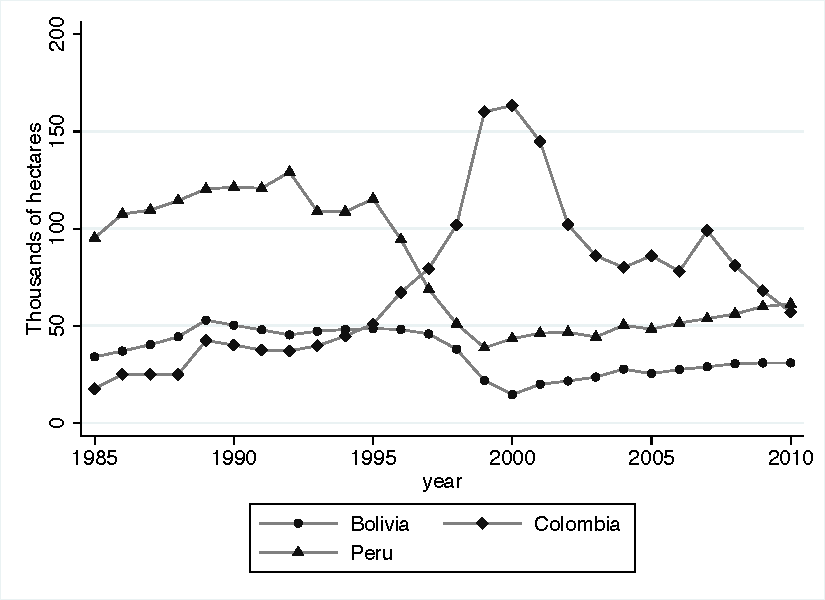
\includegraphics[scale=1]{coca_andean_region.pdf}
	\caption{Presence of coca fields in the Andean region}
	\captionsetup{font={footnotesize}}
	\caption*{Source: Author based on UNODC and U.S. State Department. Estimates for Bolivia include 12,000 hectares authorized since 1988}
	\label{ef_cocaandean}
\end{figure}


\begin{figure}[htbp]
	\centering
	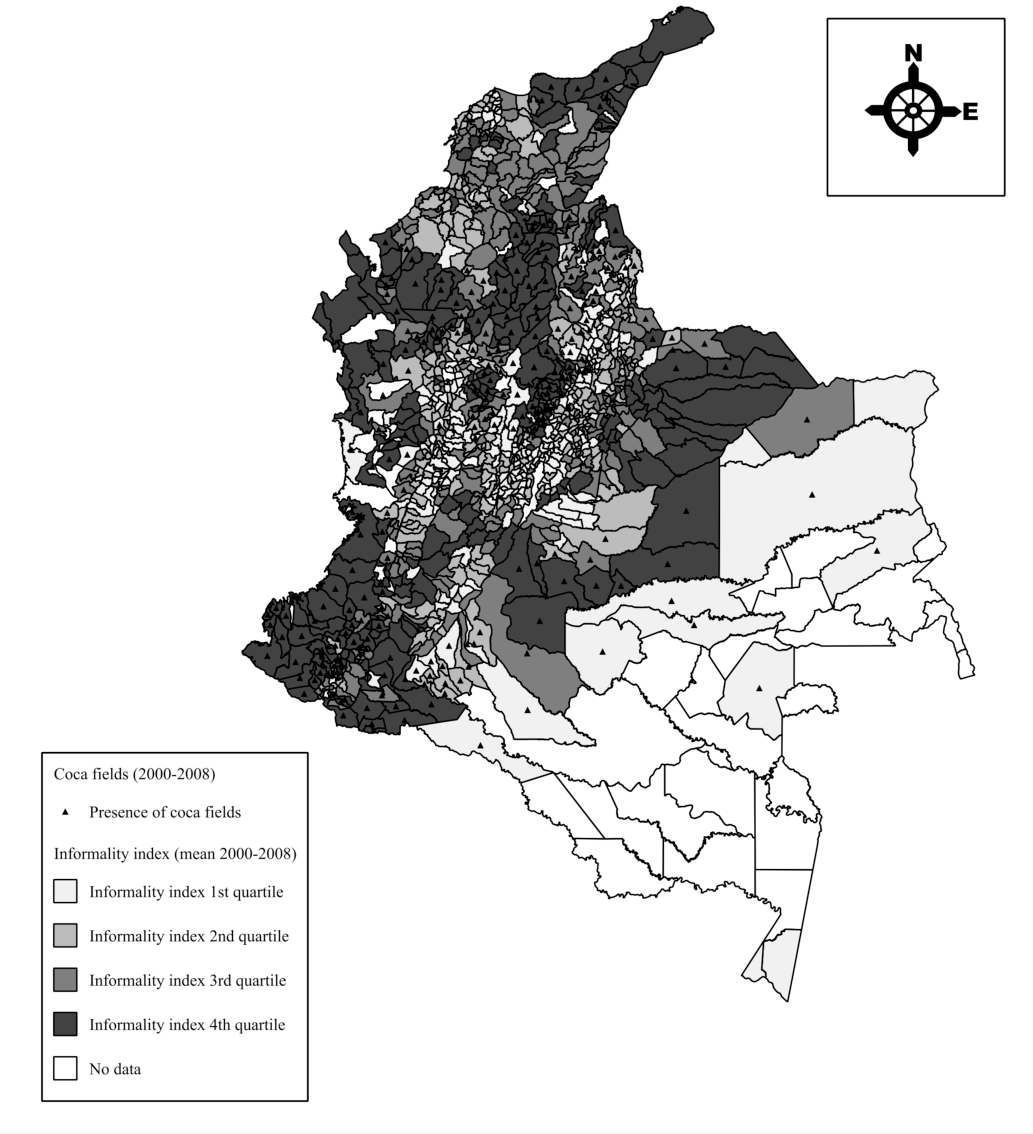
\includegraphics[scale=1]{map_colombia.pdf}
	\caption{Presence of coca fields (any year 2000-2008) and quartiles of informality index (mean 2000-2008) in Colombia}
	\captionsetup{font={footnotesize}}
	\caption*{Source: Author based on UNODC and IGAC. The figure shows municipalities that ever had presence of illicit coca leaf plantations for the period 2000 to 2008 and quartiles of the average informality index for the same period.}
	\label{ds_map}
\end{figure}


\begin{figure}[htbp]
	\centering
	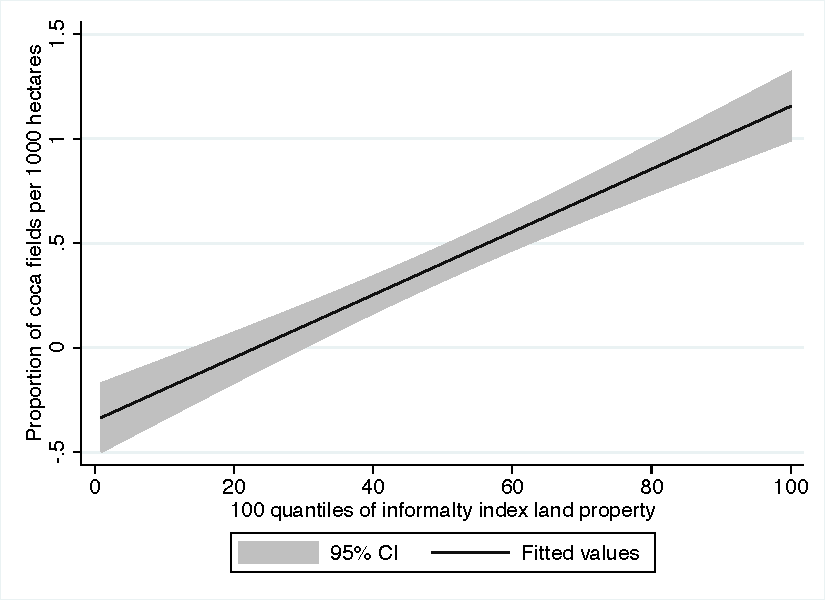
\includegraphics[scale=1]{l_fit.pdf}
	\caption{Linear fit of proportion of coca fields per 1,000 hectares and 100 quantiles of informality index}
	\captionsetup{font={footnotesize}}
	\caption*{Source: Author based on UNODC and IGAC. The linear fit includes 892 municipalities for the period 2000 to 2008.}
	\label{ds_lfit}
\end{figure}

\FloatBarrier
\newpage
\thispagestyle{empty}
\mbox{}\ 

\end{document}

